% Options for packages loaded elsewhere
\PassOptionsToPackage{unicode}{hyperref}
\PassOptionsToPackage{hyphens}{url}
\PassOptionsToPackage{dvipsnames,svgnames,x11names}{xcolor}
%
\documentclass[
  english,
  man,floatsintext]{apa7}
\title{TITLE}
\author{Sebastian Sciarra\textsuperscript{1}}
\date{}

\usepackage{amsmath,amssymb}
\usepackage{lmodern}
\usepackage{iftex}
\ifPDFTeX
  \usepackage[T1]{fontenc}
  \usepackage[utf8]{inputenc}
  \usepackage{textcomp} % provide euro and other symbols
\else % if luatex or xetex
  \usepackage{unicode-math}
  \defaultfontfeatures{Scale=MatchLowercase}
  \defaultfontfeatures[\rmfamily]{Ligatures=TeX,Scale=1}
\fi
% Use upquote if available, for straight quotes in verbatim environments
\IfFileExists{upquote.sty}{\usepackage{upquote}}{}
\IfFileExists{microtype.sty}{% use microtype if available
  \usepackage[]{microtype}
  \UseMicrotypeSet[protrusion]{basicmath} % disable protrusion for tt fonts
}{}
\makeatletter
\@ifundefined{KOMAClassName}{% if non-KOMA class
  \IfFileExists{parskip.sty}{%
    \usepackage{parskip}
  }{% else
    \setlength{\parindent}{0pt}
    \setlength{\parskip}{6pt plus 2pt minus 1pt}}
}{% if KOMA class
  \KOMAoptions{parskip=half}}
\makeatother
\usepackage{xcolor}
\IfFileExists{xurl.sty}{\usepackage{xurl}}{} % add URL line breaks if available
\IfFileExists{bookmark.sty}{\usepackage{bookmark}}{\usepackage{hyperref}}
\hypersetup{
  pdfauthor={Sebastian Sciarra1},
  pdflang={en-EN},
  pdfkeywords={measurement timing, nonlinear},
  colorlinks=true,
  linkcolor={blue},
  filecolor={Maroon},
  citecolor={Blue},
  urlcolor={Blue},
  pdfcreator={LaTeX via pandoc}}
\urlstyle{same} % disable monospaced font for URLs
\usepackage{graphicx}
\makeatletter
\def\maxwidth{\ifdim\Gin@nat@width>\linewidth\linewidth\else\Gin@nat@width\fi}
\def\maxheight{\ifdim\Gin@nat@height>\textheight\textheight\else\Gin@nat@height\fi}
\makeatother
% Scale images if necessary, so that they will not overflow the page
% margins by default, and it is still possible to overwrite the defaults
% using explicit options in \includegraphics[width, height, ...]{}
\setkeys{Gin}{width=\maxwidth,height=\maxheight,keepaspectratio}
% Set default figure placement to htbp
\makeatletter
\def\fps@figure{htbp}
\makeatother
\setlength{\emergencystretch}{3em} % prevent overfull lines
\providecommand{\tightlist}{%
  \setlength{\itemsep}{0pt}\setlength{\parskip}{0pt}}
\setcounter{secnumdepth}{5}
% Make \paragraph and \subparagraph free-standing
\ifx\paragraph\undefined\else
  \let\oldparagraph\paragraph
  \renewcommand{\paragraph}[1]{\oldparagraph{#1}\mbox{}}
\fi
\ifx\subparagraph\undefined\else
  \let\oldsubparagraph\subparagraph
  \renewcommand{\subparagraph}[1]{\oldsubparagraph{#1}\mbox{}}
\fi
\newlength{\cslhangindent}
\setlength{\cslhangindent}{1.5em}
\newlength{\csllabelwidth}
\setlength{\csllabelwidth}{3em}
\newlength{\cslentryspacingunit} % times entry-spacing
\setlength{\cslentryspacingunit}{\parskip}
\newenvironment{CSLReferences}[2] % #1 hanging-ident, #2 entry spacing
 {% don't indent paragraphs
  \setlength{\parindent}{0pt}
  % turn on hanging indent if param 1 is 1
  \ifodd #1
  \let\oldpar\par
  \def\par{\hangindent=\cslhangindent\oldpar}
  \fi
  % set entry spacing
  \setlength{\parskip}{#2\cslentryspacingunit}
 }%
 {}
\usepackage{calc}
\newcommand{\CSLBlock}[1]{#1\hfill\break}
\newcommand{\CSLLeftMargin}[1]{\parbox[t]{\csllabelwidth}{#1}}
\newcommand{\CSLRightInline}[1]{\parbox[t]{\linewidth - \csllabelwidth}{#1}\break}
\newcommand{\CSLIndent}[1]{\hspace{\cslhangindent}#1}
% Manuscript styling
\usepackage{upgreek}
\captionsetup{font=singlespacing,justification=justified}

% Table formatting
\usepackage{longtable}
\usepackage{lscape}
% \usepackage[counterclockwise]{rotating}   % Landscape page setup for large tables
\usepackage{multirow}		% Table styling
\usepackage{tabularx}		% Control Column width
\usepackage[flushleft]{threeparttable}	% Allows for three part tables with a specified notes section
\usepackage{threeparttablex}            % Lets threeparttable work with longtable

% Create new environments so endfloat can handle them
% \newenvironment{ltable}
%   {\begin{landscape}\begin{center}\begin{threeparttable}}
%   {\end{threeparttable}\end{center}\end{landscape}}
\newenvironment{lltable}{\begin{landscape}\begin{center}\begin{ThreePartTable}}{\end{ThreePartTable}\end{center}\end{landscape}}

% Enables adjusting longtable caption width to table width
% Solution found at http://golatex.de/longtable-mit-caption-so-breit-wie-die-tabelle-t15767.html
\makeatletter
\newcommand\LastLTentrywidth{1em}
\newlength\longtablewidth
\setlength{\longtablewidth}{1in}
\newcommand{\getlongtablewidth}{\begingroup \ifcsname LT@\roman{LT@tables}\endcsname \global\longtablewidth=0pt \renewcommand{\LT@entry}[2]{\global\advance\longtablewidth by ##2\relax\gdef\LastLTentrywidth{##2}}\@nameuse{LT@\roman{LT@tables}} \fi \endgroup}

% \setlength{\parindent}{0.5in}
% \setlength{\parskip}{0pt plus 0pt minus 0pt}

% Overwrite redefinition of paragraph and subparagraph by the default LaTeX template
% See https://github.com/crsh/papaja/issues/292
\makeatletter
\renewcommand{\paragraph}{\@startsection{paragraph}{4}{\parindent}%
  {0\baselineskip \@plus 0.2ex \@minus 0.2ex}%
  {-1em}%
  {\normalfont\normalsize\bfseries\itshape\typesectitle}}

\renewcommand{\subparagraph}[1]{\@startsection{subparagraph}{5}{1em}%
  {0\baselineskip \@plus 0.2ex \@minus 0.2ex}%
  {-\z@\relax}%
  {\normalfont\normalsize\itshape\hspace{\parindent}{#1}\textit{\addperi}}{\relax}}
\makeatother

% \usepackage{etoolbox}
\makeatletter
\patchcmd{\HyOrg@maketitle}
  {\section{\normalfont\normalsize\abstractname}}
  {\section*{\normalfont\normalsize\abstractname}}
  {}{\typeout{Failed to patch abstract.}}
\patchcmd{\HyOrg@maketitle}
  {\section{\protect\normalfont{\@title}}}
  {\section*{\protect\normalfont{\@title}}}
  {}{\typeout{Failed to patch title.}}
\makeatother
\shorttitle{Measurement timing}
\keywords{measurement timing, nonlinear \newline\indent Word count: 5554 words}
\usepackage{lineno}

\linenumbers
\usepackage{csquotes}
\usepackage{nccmath}
\usepackage{caption}
\usepackage{textcomp}
\usepackage{longtable}
\usepackage{makecell}
\usepackage[section]{placeins}
\usepackage{setspace}
\usepackage{biblatex}
\usepackage{booktabs}
\usepackage{array}
\usepackage{multirow}
\usepackage{wrapfig}
\usepackage{colortbl}
\usepackage{pdflscape}
\usepackage{tabu}
\usepackage{threeparttable}
\usepackage{threeparttablex}
\usepackage[normalem]{ulem}
\usepackage{xcolor}
\usepackage{amsthm}
\usepackage{amsmath}
\usepackage{bm}
\DeclareMathOperator*{\argmax}{arg\,max}
\usepackage{setspace}
\usepackage[labelfont = {bf, up}]{caption}
\newcommand{\blandscape}{\begin{landscape}}
\newcommand{\elandscape}{\end{landscape}}
\usepackage{upgreek}
\usepackage{subcaption}
\captionsetup[figure]{labelfont={normalfont, bf}, singlelinecheck=false, labelsep=newline}
\DeclareCaptionFont{figCaptionFont}{\fontfamily{phv}\doublespacing}
\DeclareCaptionFont{figCaptionSize}{\fontsize{11pt}{13.2pt}\selectfont}
\DeclareCaptionFont{tabCaptionSize}{\small}
\DeclareCaptionFont{figCaptionStyle}{\textup}
\DeclareCaptionLabelSeparator{captionSep}{\newline}
\captionsetup[figure]{labelfont={figCaptionStyle, bf}, font = {figCaptionFont,figCaptionSize, figCaptionStyle}, labelsep = captionSep, justification= raggedright}
\captionsetup[table]{labelfont={tabCaptionSize, bf}, font = {figCaptionFont, tabCaptionSize, figCaptionStyle}, labelsep = captionSep, justification= raggedright}
\newenvironment{helvenv}{\fontfamily{phv}\selectfont}{}
\raggedbottom
\usepackage{anyfontsize}
\AtBeginEnvironment{ThreePartTable}{\fontfamily{phv} \fontsize{10.5pt}{12pt}\selectfont}
\AtBeginEnvironment{tablenotes}{\fontsize{9.5pt}{11.4pt}\selectfont}
\setcounter{section}{0}
\makeatletter \renewcommand\thesection{}\renewcommand\thesubsection{\@arabic\c@section.\@arabic\c@subsection} \makeatother
\setlength\cmidrulewidth{1pt}
\setlength\lightrulewidth{1pt}
\newtheorem{theorem}{Theorem}
\newtheorem{example}[theorem]{Example}
\renewcommand\theadfont{}
\newcommand{\figurefootnote}{\raggedright\linespread{2}\fontfamily{phv}\fontsize{9.5pt}{11.4pt}\selectfont \textit{Note. }}
\makeatletter
\renewcommand{\paragraph}{\@startsection{paragraph}{4}{\parindent}%
  {0\baselineskip \@plus 0.2ex \@minus 0.2ex}%
  {-1em}%
  {\normalfont\normalsize\bfseries\typesectitle}}

\renewcommand{\subparagraph}[1]{\@startsection{subparagraph}{5}{1em}%
  {0\baselineskip \@plus 0.2ex \@minus 0.2ex}%
  {-\z@\relax}%
  {\normalfont\normalsize\bfseries\itshape\hspace{\parindent}{#1}\textit{\addperi}}{\relax}}
\makeatother

\ifXeTeX
  % Load polyglossia as late as possible: uses bidi with RTL langages (e.g. Hebrew, Arabic)
  \usepackage{polyglossia}
  \setmainlanguage[]{english}
\else
  \usepackage[main=english]{babel}
% get rid of language-specific shorthands (see #6817):
\let\LanguageShortHands\languageshorthands
\def\languageshorthands#1{}
\fi
\ifLuaTeX
  \usepackage{selnolig}  % disable illegal ligatures
\fi


\authornote{

Correspondence concerning this article should be addressed to Sebastian Sciarra. E-mail: \href{mailto:ssciarra@uoguelph.ca}{\nolinkurl{ssciarra@uoguelph.ca}}

}

\affiliation{\vspace{0.5cm}\textsuperscript{1} University of Guelph}

\begin{document}
\maketitle

\newpage
\vspace*{-\topskip}
\vspace*{\fill}
\nointerlineskip

\begin{titlepage}
  \begin{center}
    \vspace*{3cm}
    
  \textbf{Is Timing Everything? Measurement Timing and the Ability to Accurately Model Longitudinal Data}
    
  \vspace{2cm} 
    by \\ Sebastian Sciarra 
    
      
  \vspace{2cm} 
   In partial fulfilment of requirements \\ 
   for the degree of \\
   Doctor of Philosophy \\ 
   in \\ 
   Psychology
    

  \vspace{2cm} 
    Guelph, Ontario, Canada \\ 
    \textcopyright \text{ Sebastian Sciarra, September 2022}

  
  \end{center}
\end{titlepage}

\newpage
\vspace*{-\topskip}
\vspace*{\fill}
\nointerlineskip

\hypertarget{introduction}{%
\section{Introduction}\label{introduction}}

\nointerlineskip
\vfill
\newpage

``Neither the behavior of human beings nor the activities of organizations can be defined without reference to time, and temporal aspects are critical for understanding them'' (Navarro et al., 2015, p. 136).

The topic of time has received a considerable amount of
attention in organizational psychology over the past 20 years. Examples
of well-received articles published around the beginning of the 21\textsuperscript{st}
century discuss how investigating time is important for
understanding patterns of change and boundary conditions of theory
(Zaheer et al., 1999), how longitudinal research is necessary for disentangling
different types of causality (T. R. Mitchell \& James, 2001), and explicate a pattern
of organizational change (or institutionalization; Lawrence et al., 2001).
Since then, articles have emphasized the need to address time in
specific areas such as performance (Dalal et al., 2014; C. D. Fisher, 2008), teams (Roe et al., 2012), and goal setting (Fried \& Slowik, 2004) and, more generally, throughout organizational research (Aguinis \& Bakker, 2021; George \& Jones, 2000; Kunisch et al., 2017; Navarro et al., 2015; Ployhart \& Vandenberg, 2010; Roe, 2008; Shipp \& Cole, 2015; Sonnentag, 2012; Vantilborgh et al., 2018).

The importance of time has also been recognized in organizational theory. In defining a theoretical contribution, Whetten (1989) discussed that time must be discussed in regard to setting boundary conditions (i.e., under what circumstances does the theory apply) and in specifying relations between variables over time (George \& Jones, 2000; see also T. R. Mitchell \& James, 2001). Even if a considerable number of organizational theories do not adhere to the definition of Whetten (1989), theoretical models in organizational psychology consist of path diagrams that delineate the causal underpinnings of a process. Given that temporal precedence is a necessary condition for establishing causality (Mill, 2011), time has a role, whether implicitly or explicitly, in organizational theory.





Despite the considerable emphasis that has been placed on investigating processes over time and its ubiquity in organizational theory, the prevalence of longitudinal research has historically remained low. One study examined the prevalence of longitudinal research from 1970--2006 across five organizational psychology journals and found that 4\% of articles used longitudinal designs (Roe, 2014). Another survey of two applied psychology journals in 2005 found that approximaely 10\% (10 of 105 studies) of studies used longitudinal designs (Roe, 2008). Similarly, two surveys of studies employing longitudinal designs with mediation analysis found that, across five journals, only about 10\% (7 of 72 studies) did so in 2005 (Maxwell \& Cole, 2007) and approximately 16\% (15 of 92 studies) did so in 2006 (M. A. Mitchell \& Maxwell, 2013).\footnote{Note that the definition of a longitudinal design in Maxwell and Cole (2007) and M. A. Mitchell and Maxwell (2013) required that measurements be taken over at least three time points so that measurements of the predictor, mediator, and outcome variables were separated over time.} Thus, the prevalence of longitudinal research has remained low.

In the six sections that follow, I will explain why longitudinal research is necessary and the factors that must be considered when conducting such research. In the first section, I will explain why conducting longitudinal research is essential for understanding the dynamics of psychological processes. In the second section, I will overview patterns of change that are likely to emerge over time. In the the third section, I will overview design and analytical issues involved in designing longitudinal studies. In the fourth section, I will explain how design and analytical issues encountered in conducting longitudinal research can be investigated. In the fifth section, I will provide a systematic review of the research that has investigated design and analytical issues involved in conducting longitudinal research. Finally, in the sixth section, I will briefly explain strategies for modelling nonlinear change. A summary of the three simulation experiments that I conducted in my dissertation will then be provided.

\hypertarget{the-need-to-conduct-longitudinal-research}{%
\subsection{The Need to Conduct Longitudinal Research}\label{the-need-to-conduct-longitudinal-research}}

Longitudinal research provides substantial advantages over cross-sectional research. Unfortunately, researchers commonly discuss the results of cross-sectional analyses as if they have been obtained with a longitudinal design. However, cross-sectional and longitudinal analyses often produce different results. Oneexample of the assumption that cross-sectional findings are equivalent to longitudinal findings comes from the large number of studies employing mediation analysis. Given that mediation is used to understand chains of causality in psychological processes (Baron \& Kenny, 1986), it would thus make sense to pair mediation analysis with a longitudinal design because understanding causality, after all, requires temporal precedence. Unfortunately, the majority of studies that have used mediation analysis have done so using cross-sectional designs---with estimates of approximately 90\% (Maxwell \& Cole, 2007) and 84\% (M. A. Mitchell \& Maxwell, 2013)---and have often discussed the results as if they were longitudinal. Investigations into whether mediation results remain equivalent across cross-sectional and longitudinal designs have repeatedly concluded that using mediation analysis on cross-sectional data can return different, and sometimes completely opposite, results from using it on longitudinal data (Cole \& Maxwell, 2003; Maxwell et al., 2011; Maxwell \& Cole, 2007; M. A. Mitchell \& Maxwell, 2013; O'Laughlin et al., 2018). Therefore, mediation analyses based on cross-sectional analyses may be misleading.

The non-equivalence of cross-sectional and longitudinal results that occurs with mediation analysis is, unfortunately, not due to a specific set of circumstances that only arise with mediation analysis, but a consequence of a broader systematic cause that affects the results of almost every analysis. The concept of ergodicity explains why cross-sectional and longitudinal analyses seldom yield similar results. To understand ergodicity, it is first important to realize that variance is central to many statistical analyses---correlation, regression, factor analysis, and mediation are some examples. Thus, if variance remains unchanged across cross-sectional and longitudinal data sets, then analyses of either data set would return the same results. Importantly, variance only remains equal across cross-sectional and longitudinal data sets if two conditions put forth by ergodic theory are satisfied (homogeneity and stationarity; Molenaar, 2004; Molenaar \& Campbell, 2009). If these two conditions are met, then a process is said to be ergodic. Unfortunately, the two conditions required for ergodicity are highly unlikely to be satisfied and so cross-sectional findings will frequently deviate from longitudinal findings (see {[}Technical Appendix A{]}{[}Technical Appendix A: Ergodicity and the Need to Conduct Longitudinal Research{]} for more information).



Given that cross-sectional and longitudinal analyses are, in general, unlikely to return equivalent findings, it is unsurprising that several investigations in organizational research---and psychology as a whole---have found these analyses to return different results. Beginning with an example from Curran and Bauer (2011), heart attacks are less likely to occur in people who exercise regularly (longitudinal finding), but more likely to happen when exercising (cross-sectional finding). Correlational studies find differences in correlation magnitudes between cross-sectional and longitudinal data sets J. Fisher et al. (2018).\footnote{Note that J. Fisher et al. (2018) also found the variability of longitudinal correlations to be considerably larger than the variability of cross-sectional correlations.} Moving on to perhaps the most commonly employed analysis in organizational research of mediation, several articles have highlighted cross-sectional data can return different, and sometimes completely opposite, results to longitudinal data (Cole \& Maxwell, 2003; Maxwell et al., 2011; Maxwell \& Cole, 2007; O'Laughlin et al., 2018). Factor analysis is perhaps the most interesting example: The well-documented five-factor model of personality seldom arises when analyzing person-level data that was obtained by measuring personality on 90 consecutive days (Hamaker et al., 2005). Therefore, cross-sectional analyses are rarely equivalent to longitudinal analyses.

Fortunately, technological advancements have allowed researchers to more easily conduct longitudinal research in two ways. First, the use of the experience sampling method (Beal, 2015) in conjunction with modern information transmission technologies---whether through phone applications or short message services---allows data to sometimes be sampled over time with relative ease. Second, the development of analyses for longitudinal data (along with their integration in commonly used software) that enable person-level data to be modelled such as multilevel models (Raudenbush \& Bryk, 2002), growth mixture models (Mo Wang \& Bodner, 2007), and dynamic factor analysis (Ram et al., 2013) provide researchers with avenues to explore the temporal dynamics of psychological processes. With one recent survey estimating that 43.3\% of mediation studies (26 of 60 studies) used a longitudinal design (O'Laughlin et al., 2018), it appears that the prevalence of longitudinal research has increased from the 9.5\% (Roe, 2008) and 16.3\% (M. A. Mitchell \& Maxwell, 2013) values estimated at the beginning of the 21\textsuperscript{st} century. Although the frequency of longitudinal research appears to have increased over the past 20 years, several avenues exist where the quality of longitudinal research can be improved, and in my dissertation, I focus on investigating these avenues.

\hypertarget{understanding-patterns-of-change-that-emerge-over-time}{%
\subsection{Understanding Patterns of Change That Emerge Over Time}\label{understanding-patterns-of-change-that-emerge-over-time}}

Change can occur in many ways over time. One pattern of change commonly assumed to occur over time is that of linear change. When change follows a linear pattern, the rate of change over time remains constant. Unfortunately, a linear pattern places demanding restrictions on possible patterns of change. If change were to follow a linear pattern, then any pauses in change (or plateaus) or changes in direction would not occur and effects would simply grow over time. Unfortunately, effect sizes have been shown to diminish over time (for meta-analytic examples, see Cohen, 1993; Griffeth et al., 2000; Hom et al., 1992; Riketta, 2008; Steel et al., 1990; Steel \& Ovalle, 1984). Moreover, many variables display cyclic patterns of change over time, with mood (Larsen \& Kasimatis, 1990), daily stress (Bodenmann et al., 2010), and daily drinking behaviour (Huh et al., 2015) as some examples. Therefore, change over is unlikely to follow a linear pattern.

A more realistic pattern of change to occur over time is a nonlinear pattern (for a review, see Cudeck \& Harring, 2007). Nonlinear change allows nonconstant rates of change such that change may occur more rapidly during certain periods of time, stop altogether, or reverse direction. When looking at patterns of change observed across psychology, examples appear in the declining rate of speech errors throughout child development (Burchinal \& Appelbaum, 1991), forgetting rates in memory (Murre \& Dros, 2015), development of habits over time (Fournier et al., 2017), and the formation of opinions over time (Xia et al., 2020). Given nonlinear change appears more likely than linear change, my dissertation will assume change over time to be nonlinear.

\hypertarget{challenges-involved-in-conducting-longitudinal-research}{%
\subsection{Challenges Involved in Conducting Longitudinal Research}\label{challenges-involved-in-conducting-longitudinal-research}}



Conducting longitudinal research presents researchers with several challenges. Many challenges are those from cross-sectional research only amplified (for a review, see Bergman \& Magnusson, 1990).\footnote{It should be noted that conducting a longitudinal study does alleviate some issues encountered in conducting cross-sectional research. For example, taking measurements over multiple time points likely reduces common method variance (Podsakoff et al., 2003; for an example, see Ostroff et al., 2002).} For example, greater efforts have to be made to to prevent missing data which can increase over (Dillman et al., 2014; Newman, 2008). Likewise, the adverse effects of well-documented biases such as demand characteristics (Orne, 1962) and social desirability (Nederhof, 1985) have to be countered at each time point. Outside challenges share with cross-sectional research, conducting longitudinal research also presents new challenges. Analyses of longitudinal data have to consider complications such as how to model error structures (Grimm \& Widaman, 2010), check for measurement non-invariance over time (the extent to which a construct is measured with equivalent accuracy over time; Schoot et al., 2012), and how to center/process data to appropriately answer research questions (Enders \& Tofighi, 2007; Wang \& Maxwell, 2015).

Although researchers must contend with several issues in conducting longitudinal research, three issues are of particular interest in my dissertation. The first issue concerns how many measurements to use in a longitudinal design. The second issue concerns how to space the measurements. The third issue focuses on how much error is incurred if the time structuredness of the data is overlooked. The sections that follow will review each of these issues.

\hypertarget{number-of-measurements}{%
\subsubsection{Number of Measurements}\label{number-of-measurements}}

Researchers have to decide on the number of measurements to include in a longitudinal study. Although using more measurements increases the accuracy of results---as noted in the results of several studies (e.g., Coulombe et al., 2016; Finch, 2017; Fine et al., 2019; Timmons \& Preacher, 2015)---taking additional measurements often comes at a cost that a researcher may be unable account for with a limited budget. One important point to mention is that a researcher designing a longitudinal study must take at least three measurements to obtain a reliable estimate of change and, perhaps more importantly, to allow a nonlinear pattern of change to be modelled (Ployhart \& Vandenberg, 2010). In my dissertation, I hope to determine whether an optimal number of measurements exists when modelling a nonlinear pattern of change.

\hypertarget{spacing-of-measurements}{%
\subsubsection{Spacing of Measurements}\label{spacing-of-measurements}}

Additionally, a researcher must decide on the spacing of measurements in a longitudinal study. Although discussions of measurement spacing often recommend that researchers use theory and previous studies to implement measurement spacings that Dormann \& Griffin (2015), organizational theories seldom delineate a period of time over which a process unfolds, and so the majority of longitudinal research uses intervals of convention and/or convenience to space measurements (Dormann \& Ven, 2014; T. R. Mitchell \& James, 2001). Unfortunately, using measurement spacing lengths that do not account for the temporal pattern of change of a psychological process can lead to inaccurate results (e.g., Chen et al., 2014). As an example, Cole and Maxwell (2009) provide show how correlation magnitudes are affected by the choice of measurement spacing intervals. In my dissertation, I hope to determine whether an optimal measurement spacing schedule exists when modelling a nonlinear pattern of change.

\hypertarget{time-structuredness}{%
\subsubsection{Time Structuredness}\label{time-structuredness}}

Last, and perhaps most pernicious, analyses of longitudinal data are likely to incur error from an assumption they make about data collection conditions. Many analyses assume that, across all collection points, participants provide their data at the same time. Unfortunately, such a high level of regularity in the response patterns of participants is unlikely: Participants are more likely to provide their data over some period of time after a data collection window has opened. As an example, consider a study that collects data from participants at the beginning of each month. If participants respond with perfect regularity, then they would all provide their data at the exact same time (e.g., noon on the second day of each month). If the participants respond with imperfect regularity, then they would provide their at different times after the beginning of each month. The regularity of responding observed across participants in a longitudinal study determines the time structuredness of the data and the sections that follow will provide overview of time structuredness.

\hypertarget{time-structured-data}{%
\paragraph{Time-Structured Data}\label{time-structured-data}}



Many analyses assume that data are \emph{time structured}: Participants provide data at the same time at each collection point. By assuming time-structured data, an analysis can incur error because it will map time intervals of inappropriate lengths onto the time intervals that occurred between participant's responses.\footnote{It should be noted that, although seldom implemented, analyses can be accessorized to handle time-unstructured data by using definition variables (Mehta \& Neale, 2005; Mehta \& West, 2000).} As an example of the consequences of incorrectly assuming data to be time structured, consider a study that assessed the effects of an intervention on the development of leadership by collecting leadership ratings at four time points each separated by four weeks (Day \& Sin, 2011). The employed analysis assumed time-structured data; that is, each each participant provided ratings on the same day---more specifically, the exact same moment---each time these ratings were collected. Unfortunately, it is unlikely that the data collected from participants were time structured: At any given collection point, some participants may have provided leadership ratings at the beginning of the week, while others may only provide ratings two weeks after the survey opened. Importantly, ratings provided two weeks after the survey opened were likely influenced by changes in leadership that occurred over the two weeks. If an analysis incorrectly assumes time-structured data, then it assumes each participant has the same response rate and, therefore, will incorrectly attribute the amount of time that elapses between most participants' responses. For instance, if a participant only provides a leadership rating two weeks after having received a survey (and six weeks after providing their previous rating), then using an analysis that assumes time-structured data would incorrectly assume that each collection point of this participant is separated by four weeks (the interval used in the experiment) and would, consequently, model the observed change as if it had occurred over four weeks. Therefore, incorrectly assuming data to be time structured leads an analysis to overlook the unique response rates of participants across the collection points and, as a consequence, incur error (Coulombe et al., 2016; Mehta \& Neale, 2005; Mehta \& West, 2000).

\hypertarget{time-unstructured-data}{%
\paragraph{Time-Unstructured Data}\label{time-unstructured-data}}

Conversely, some analyses assume that data are \emph{time unstructured}: Participants provide data at different times at each collection point. Given the unlikelihood of one response pattern describing the response rates of all participants in a given study, the data
obtained in a study are unlikely to be time structured. Instead, and because participants are likely to exhibit unique response
patterns in their response rates, data are likely to be time unstructured. One way to conceptualize the distinction between time-structured and time-unstructured data is on a continuum. On one end of the continuum, participants all provide data with identical response patterns, thus giving time-structured data. When participants show unique response patterns, the resulting data are time unstructured, with the extent of time-unstructuredness depending on the length of the response windows. For example, if data are collected at the beginning of each month and participants only have one day to provide data at each time, then, assuming a unique response rate for each participant, the resulting data will have a low amount of time unstructuredness. Alternatively, if data are collected at the beginning of each month and participants have 30 days to provide data each time, then, assuming a unique response rate for each participant, the resulting data will have a high amount of time unstructuredness. Therefore, the continuum of time struturedness has time-structured data on one end and time-unstructured data with long response rates on another end. In my dissertation, I hope to determine how much error is incurred when time-unstructured data are assumed to be time structured.

\hypertarget{summary}{%
\subsubsection{Summary}\label{summary}}

In summary, researchers must contend with several issues when conducting longitudinal research. In addition to contending with issues encountered in conducting cross-sectional research, researchers must contend with new issues that arise from conducting longitudinal research. Three issues of particular importance in my dissertation are the number of measurements, the spacing of measurements, and incorrectly assuming data to be time structured. These issues will be serve as a basis for a systematic review of the simulation literature.

\hypertarget{using-simulations-to-assess-modelling-accuracy}{%
\subsection{Using Simulations To Assess Modelling Accuracy}\label{using-simulations-to-assess-modelling-accuracy}}

In the next section, I will present the results of the systematic review of the literature that has investigated the issues of measurement number, measurement spacing, and time structuredness. Before presenting the results of the systematic review, I will provide an overview of the Monte Carlo method used to investigate issues involved in conducting longitudinal research.

To understand how the effects of longitudinal issues on modelling accuracy can be investigated, the inferential method commonly employed in psychological research will first be reviewed with an emphasis on its shortcomings (see Figure \ref{fig:MonteCarlo-comparison}). Consider an example where a researcher wants to estimate a population mean (\(\upmu\)) and understand how sampling error affects the accuracy of the estimate. Using the inferential method, the researcher samples data and then estimates the population mean (\(\upmu\)) by computing the mean of the sampled data. Because collected samples are almost always contaminated by a variety of methodological and/or statistical deficiencies (such as sampling error, measurement error, assumption violations, etc.), the estimation of the population parameter is likely to be imperfect. Unfortunately, to estimate the effect of sampling error on the accuracy of the population mean estimate (\(\upmu\)), the researcher would need to know the value of the population mean; without knowing the value of the population mean, it is impossible to know how much error was incurred in estimating the population mean and, as as a result, impossible to know the extent to which sampling error contributed to this error. Therefore, a study following the inferential approach can only provide estimates of population parameters.

The Monte Carlo method has a different goal. Whereas inferential methods focus on estimating parameters from sample data, the Monte Carlo method is used to understand the factors that influence the accuracy of the inferential approach. Figure \ref{fig:MonteCarlo-comparison} shows that the Monte Carlo method works in the opposite direction of the inferential approach: Instead of collecting a sample, the Monte Carlo method begins by assigning a value to at least one parameter to define a population. Many sample data sets are then generated from the defined population, with some methodological deficiency built in to each data set. In the current example, each data set is generated to have a specific amount of missing data. Each generated sample is then analyzed and the population estimates of each statistical model are averaged and compared to the pre-determined parameter value.\footnote{A statistical deficiency can also be introduced in the analysis of each generated data set.} The difference between the average of the estimates and the known population value constitutes bias in parameter estimation (i.e., parameter bias). In the current example, the missing data manipulation causes a systematic underestimation, on average, of the population parameter. By randomly generating data, the Monte Carlo method can determine how a variety of methodological and statistical factors affect the accuracy of a model (for a review, see Robert \& Casella, 2010).

\begin{figure}[H]
  \caption[Monte Carlo method]{Depiction of Monte Carlo Method}
  \label{fig:MonteCarlo-comparison}
  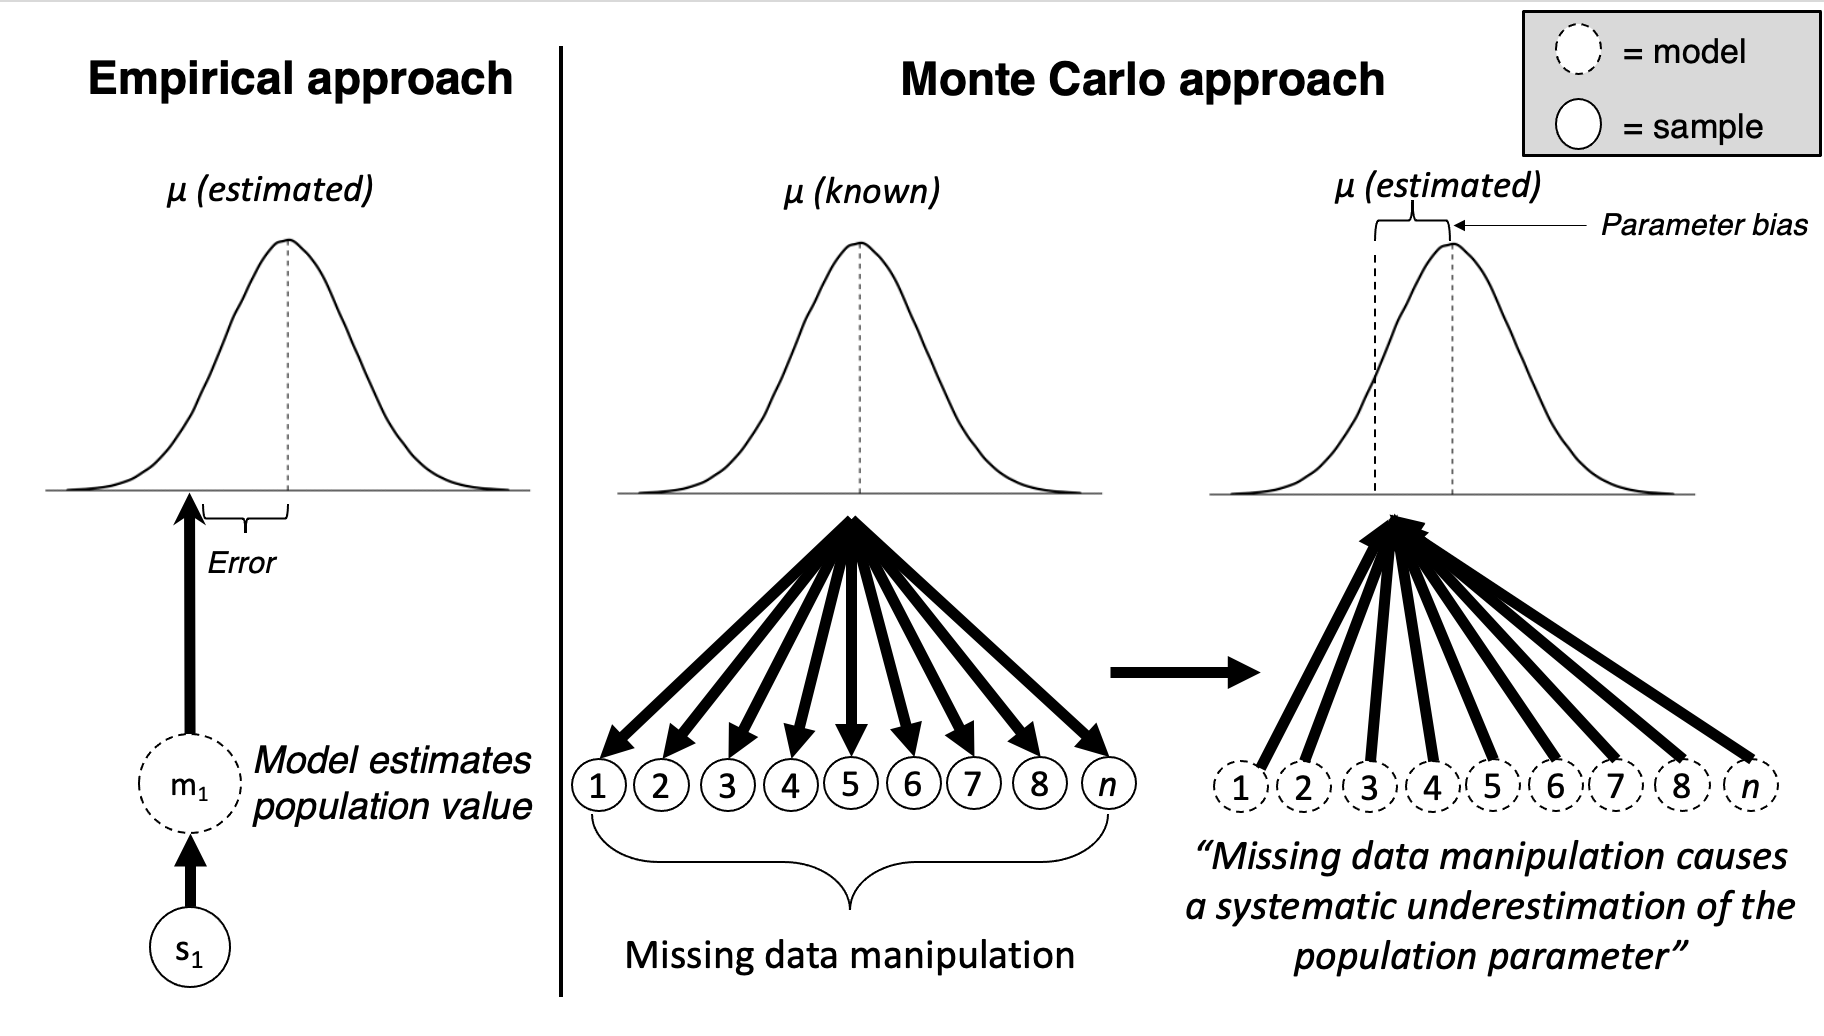
\includegraphics{Figures/Monte_Carlo_comparison} \hfill{}
    \figurefootnote{Comparison of inferential approach with the Monte Carlo approach. The inferential approach begins with a collected sample and then estimates the population parameter using an appropriate statistical model. The difference between the estimated and population value can be conceptualized as error. Because the population value is generally unknown in the inferential approach, it cannot estimate how much error is introduced by any given methodological or statistical deficiency. To estimate how much error is introduced by any given methodological or statistical deficiency, the Monte Carlo method needs to be used, which constitutes four steps. The Monte Carlo method first defines a population by setting parameter values. Second, many samples are generated from the pre-defined population, with some methodological deficiency built in to each data set (in this case, each sample has a specific amount of missing data). Third, each generated sample is then analyzed and the population estimates of each statistical model are averaged and compared to the pre-determined parameter value. Fourth, the difference between the estimate average and the known population value defines the extent to which the missing data manipulation affected parameter estimation (the difference between the population and average estimated population value is the parameter bias).}
\end{figure}

Monte Carlo simulations have been used to evaluate a variety of methodological and statistical deficiencies. Beginning with the simple bivariate correlation, Monte Carlo simulations have shown that realistic values of sample size and measurement accuracy produce considerable variability in estimated correlation values (Stanley \& Spence, 2014). Monte Carlo simulations have also provided valuable insights into more complicated statistical analyses. In investigating more complex statistical analyses, simulations have shown that mediation analyses are biased to produce results of complete mediation because the statistical power to detect direct effects falls well below the statistical power to detect indirect effects (Kenny \& Judd, 2014). Finally, as an example of the utility of Monte Carlo simulations for evaluating growth mixture models, Monte Carlo simulations have shown that class enumeration accuracy (the ability to identify the correct number of response groups) decreases with nonnormal data (Bauer, 2003). Given the ability of the Monte Carlo method to evaluate statistical methods, the experiments in my dissertation used it to evaluate the effects of measurement number, measurement spacing, and time structuredness on modelling accuracy.\footnote{My simulation experiments also investigated the effects of sample size and nature of change on modelling accuracy.}

\hypertarget{systematic-review-of-simulation-literature}{%
\subsection{Systematic Review of Simulation Literature}\label{systematic-review-of-simulation-literature}}

To understand the extent to which issues involved in conducting longitudinal research had been investigated, I conducted a systematic review of the simulation literature. The sections that follow will first present the method I followed in systematically reviewing the literature and then summarize the findings of the review.

\hypertarget{systematic-review-methodology}{%
\subsubsection{Systematic Review Methodology}\label{systematic-review-methodology}}

I identified the following keywords through citation searching and independent reading: ``growth curve,'' ``time-structured analysis,'' ``time structure,'' ``temporal design,'' ``individual measurement occasions,'' ``measurement intervals,'' ``methods of timing,'' ``longitudinal data analysis,'' ``individually-varying time points,'' ``measurement timing,'' ``latent difference score models,'' ``parameter bias,'' and ``measurement spacing.'' I entered these keywords entered into the PsycINFO database (on July 23, 2021) and any paper that contained any one of these key words and the word ``simulation'' in any field was considered a viable paper (see Figure \ref{fig:prismaDiagram} for a PRISMA diagram illustrating the filtering of the reports). The search returned 165 reports, which I screened by reading the abstracts. Initial screening led to the removal of 60 reports because they did not contain any simulation experiments. Of the remaining 105 papers, I removed 2 more popers because they could not accessed (Stockdale, 2007; Tiberio, 2008). Of the remaining 103 identified simulation studies, I deemed a paper as relevant if it investigated the effects of any design and/or analysis factor relating to conducting longitudinal research (i.e., number of measurements, spacing of measurements, and/or time structuredness) and did so using the Monte Carlo simulation method. Of the remaining 103 studies, I removed 89 studies being removed because they did not meet the inclusion criteria, leaving fourteen studies to be included the review, with. I also found an additional 3 studies through citation searching, giving a total of 17 studies.








The findings of my systematic review are summarized in Tables \ref{tab:systematicReviewCount}--\ref{tab:systematicReview}. Tables \ref{tab:systematicReviewCount}--\ref{tab:systematicReview} differ in one way: Table \ref{tab:systematicReviewCount} indicates how many studies investigated each effect, whereas Table \ref{tab:systematicReview} provides the reference of each study and detailed information about each study's method. Otherwise, all other details of Tables \ref{tab:systematicReviewCount}--\ref{tab:systematicReview} are identical. The first column lists the longitudinal design factor (alongside with sample size) and the corresponding two- and three-way interactions. The second and third columns list whether each effect has been investigated with linear and nonlinear patterns of change, respectively. Shaded cells indicate effects that have not been investigated, with cells shaded in light blue indicating effects that have not been investigated with linear patterns of change and cells shaded in dark blue indicating effects that have not been investigated with nonlinear patterns of change.\footnote{Table \ref{tab:systematicReview} lists the effects that each study (identified by my systematic review) investigated and notes the following methodological details (using superscript letters and symbols): the type
of model used in each paper, assumption and/or manipulation of complex error structures
(heterogeneous variances and/or correlated residuals), manipulation of missing data,
and/or pseudo-time structuredness manipulation. Across all 17 simulation studies, 5 studies (29\%) assumed complex error structures (Gasimova et al., 2014; Liu \& Perera, 2021; Y. Liu et al., 2015; Miller \& Ferrer, 2017; Murphy et al., 2011), 1 study (6\%) manipulated missing data (Fine et al., 2019), and 2 studies (12\%) contained a pseudo-time structuredness manipulation (Fine et al., 2019; Fine \& Grimm, 2020) . Importantly, the pseudo-time structuredness manipulation used in Fine et al. (2019) and Fine and Grimm (2020) differed from the manipulation of time
structuredness used in the current experiments (and from previous simulation experiments of Coulombe et al., 2016; Miller \& Ferrer, 2017) in that it randomly generated longitudinal data such that a given person could provide all their data before another person provided any data.}

\begin{figure}[H]
  \caption{PRISMA Diagram Showing Study Filtering Strategy}
  \label{fig:prismaDiagram}
  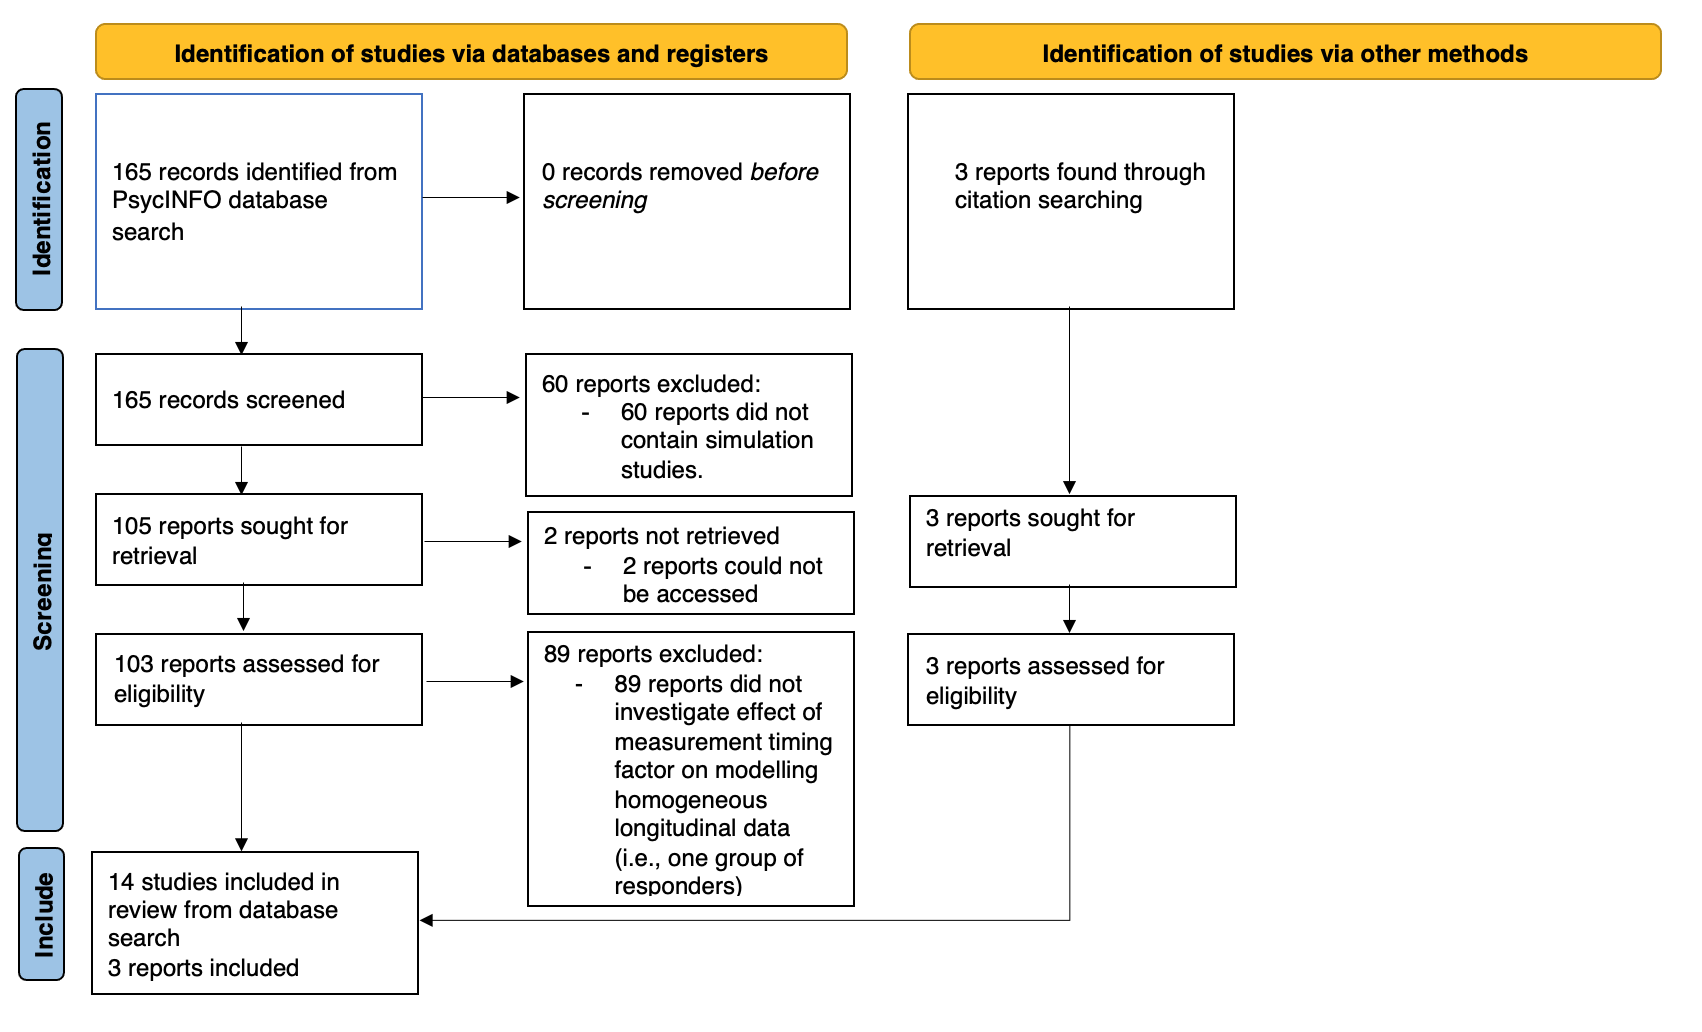
\includegraphics{Figures/prisma_diagram} \hfill{}
    \figurefootnote{PRISMA diagram for systematic review of simulation research that investigates measurement timing.}
\end{figure}

\hypertarget{systematic-review-results}{%
\subsubsection{Systematic Review Results}\label{systematic-review-results}}

Although the previous research appeared to sufficiently fill some cells of Table \ref{tab:systematicReviewCount}, two patterns suggest that arguably the most important cells (or effects) have not been investigated. First, it appears that simulation research has invested more effort in investigating the effects of longitudinal design factors with linear patterns than with nonlinear patterns of change. In counting the number of effects that remain unaddressed with linear and nonlinear patterns of change, a total of five cells (or effects) have not been

\newgeometry{margin=2.54cm}
\begin{landscape}
\begin{ThreePartTable}
\begin{TableNotes}[para]
\item \textit{\textit{Note.\hspace{-1.2pc}}} 
\item Cells are only numbered for effects that have not been investigated. Cells shaded in light blue indicate effects that have not been investigated with linear patterns of change and cells shaded in dark blue indicate effects that have not been investigated with nonlinear patterns of change.
\end{TableNotes}
\begin{longtable}[l]{>{\raggedright\arraybackslash}p{4.5cm}>{\centering\arraybackslash}p{8cm}>{\centering\arraybackslash}p{8cm}}
\caption{\label{tab:systematicReviewCount}Number of Simulation Studies That Have Investigated Longitudinal Issues with Linear and Nonlinear Change Patterns (\textit{n} = 17)}\\
\toprule
Effect & Linear pattern & Nonlinear pattern\\
\midrule
\endfirsthead
\caption[]{\label{tab:systematicReviewCount}Number of Simulation Studies That Have Investigated Longitudinal Issues with Linear and Nonlinear Change Patterns (\textit{n} = 17) \textit{(continued)}}\\
\toprule
Effect & Linear pattern & Nonlinear pattern\\
\midrule
\endhead

\endfoot
\bottomrule
\insertTableNotes
\endlastfoot
\textbf{Main effects} & \cellcolor{white}{} & \cellcolor{white}{}\\
\cmidrule{1-3}
Number of measurements (NM) & \cellcolor{white}{11 studies} & \cellcolor{white}{6 studies}\\
 
Spacing of measurements (SM) & \cellcolor{white}{1 study} & \cellcolor{white}{1 study}\\
 
Time structuredness (TS) & \cellcolor{white}{2 studies} & \cellcolor{white}{1 study}\\
 
Sample size (S) & \cellcolor{white}{11 studies} & \cellcolor{white}{7 studies}\\
\cmidrule{1-3}
\textbf{Two-way interactions} & \cellcolor{white}{} & \cellcolor{white}{}\\
\cmidrule{1-3}
NM x SM & \cellcolor{white}{1 study} & \cellcolor{white}{1 study}\\
 
NM x TS & \cellcolor{white}{1 study} & \cellcolor[HTML]{9fc5e8}{\textbf{Cell 1 (\hyperref[Exp3]{Exp. 3})}}\\
 
NM x S & \cellcolor{white}{9 studies} & \cellcolor{white}{5 studies}\\
 
SM x TS & \cellcolor[HTML]{acddfa}{\textbf{Cell 2}} & \cellcolor[HTML]{9fc5e8}{\textbf{Cell 3}}\\
 
SM x S & \cellcolor[HTML]{acddfa}{\textbf{Cell 4}} & \cellcolor[HTML]{9fc5e8}{\textbf{Cell 5 (\hyperref[Exp2]{Exp. 2})}}\\
 
TS x S & \cellcolor{white}{1 study} & \cellcolor{white}{2 studies}\\
\cmidrule{1-3}
\textbf{Three-way interactions} & \cellcolor{white}{} & \cellcolor{white}{}\\
\cmidrule{1-3}
NM x SM x TS & \cellcolor[HTML]{acddfa}{\textbf{Cell 6}} & \cellcolor[HTML]{9fc5e8}{\textbf{Cell 7}}\\
 
NM x SM x S & \cellcolor[HTML]{acddfa}{\textbf{Cell 8}} & \cellcolor[HTML]{9fc5e8}{\textbf{Cell 9 (\hyperref[Exp2]{Exp. 2})}}\\
 
NM x TS x S & \cellcolor{white}{1 study} & \cellcolor[HTML]{9fc5e8}{\textbf{Cell 10 (\hyperref[Exp3]{Exp. 3})}}\\
 
SM x TS x S & \cellcolor[HTML]{acddfa}{\textbf{Cell 11}} & \cellcolor[HTML]{9fc5e8}{\textbf{Cell 12}}\\*
\end{longtable}
\end{ThreePartTable}
\end{landscape}
\restoregeometry





































\newgeometry{margin=2.2cm}
\begin{landscape}
\begin{ThreePartTable}
\begin{TableNotes}[para]
\item \textit{\textit{Note.\hspace{-1.2pc}}} 
\item Cells are only numbered for effects that have not been investigated. Cells shaded in light and dark blue indicate effects that have not, respectively, been investigated with linear and nonlinear patterns of change.
\item \textit{\newline} 
\item[a] Latent growth curve model. \textsuperscript{b} Second-order latent growth curve model. \textsuperscript{c} Hierarchical Bayesian model. \textsuperscript{d} Bivariate latent change score model. \textsuperscript{e} Functional mixed-effects model. \textsuperscript{f} Nonlinear mixed-effects model. \textsuperscript{g} Bilinear spline model. \textsuperscript{g} Parallel bilinear spline model.
\item \textit{\newline} 
\item[$\circ$] Manipulated missing data. $^\mho$ Assumed complex error structure (heterogeneous variances and/or correlated residuals). $^\triangledown$ Contained pseudo-time structuredness manipulation.
\end{TableNotes}
\begin{longtable}[l]{l>{\centering\arraybackslash}p{8cm}>{\centering\arraybackslash}p{8cm}}
\caption{\label{tab:systematicReview}Summary of Simulation Studies That Have Investigated Longitudinal Issues with Linear and Nonlinear Change Patterns (\textit{n} = 17)}\\
\toprule
Effect & Linear pattern & Nonlinear pattern\\
\midrule
\endfirsthead
\caption[]{\label{tab:systematicReview}Summary of Simulation Studies That Have Investigated Longitudinal Issues with Linear and Nonlinear Change Patterns (\textit{n} = 17) \textit{(continued)}}\\
\toprule
Effect & Linear pattern & Nonlinear pattern\\
\midrule
\endhead

\endfoot
\bottomrule
\insertTableNotes
\endlastfoot
\textbf{Main effects} & \cellcolor{white}{} & \cellcolor{white}{}\\
\cmidrule{1-3}
Number of measurements (NM) & \cellcolor{white}{Timmons and Preacher (2015)\textsuperscript{a}; Murphy et al. (2011)$^{\mho}$\textsuperscript{b}; Gasimova et al. (2014)\textsuperscript{c}$^{\mho}$; Wu et al. (2014)\textsuperscript{a}; Coulombe (2016)\textsuperscript{a};Ye (2016)\textsuperscript{a}; Finch (2017)\textsuperscript{a}; O'Rourke et al. (2021)\textsuperscript{d}; Newsom and Smith (2020)\textsuperscript{a}; Coulombe et al. (2016)\textsuperscript{a}} & \cellcolor{white}{Timmons and Preacher (2015)\textsuperscript{a}; Finch (2017)\textsuperscript{a}; Fine et al. (2019)\textsuperscript{e}$^{\circ\triangledown}$; Fine and Grimm (2020)\textsuperscript{e,f}$^{\triangledown}$;J. Liu et al. (2019)\textsuperscript{g}; Liu and Perera (2021)\textsuperscript{h}$^{\mho}$; Y. Liu et al. (2015)\textsuperscript{g}$^{\mho}$}\\
 
Spacing of measurements (SM) & \cellcolor{white}{Timmons and Preacher (2015)\textsuperscript{a}} & \cellcolor{white}{Timmons and Preacher (2015)\textsuperscript{a}}\\
 
Time structuredness (TS) & \cellcolor{white}{Aydin et al. (2014)\textsuperscript{a}; Coulombe et al. (2016)\textsuperscript{a}} & \cellcolor{white}{Miller and Ferrer (2017)\textsuperscript{a}$^{\mho}$; Y. Liu et al. (2015)\textsuperscript{g}$^{\mho}$}\\
 
Sample size (S) & \cellcolor{white}{Murphy et al. (2011)\textsuperscript{b}${\mho}$; Gasimova et al. (2014)\textsuperscript{c}$^{\mho}$; Wu et al. (2014)\textsuperscript{a}; Coulombe (2016)\textsuperscript{a};Ye (2016)\textsuperscript{a}; Finch (2017)\textsuperscript{a}; O'Rourke et al. (2021)\textsuperscript{d}; Newsom and Smith (2020)\textsuperscript{a}; Coulombe et al. (2016)\textsuperscript{a};Aydin et al. (2014)\textsuperscript{a}; Coulombe et al. (2016)\textsuperscript{a}} & \cellcolor{white}{Finch (2017)\textsuperscript{a}; Fine et al. (2019)\textsuperscript{e}$^{\circ\triangledown}$; Fine and Grimm (2020)\textsuperscript{e,f}$^{\triangledown}$;J. Liu et al. (2019)\textsuperscript{g}; Liu and Perera (2021)\textsuperscript{h}$^{\mho}$; Y. Liu et al. (2015)\textsuperscript{g}$^{\mho}$; Miller and Ferrer (2017)\textsuperscript{a}$^{\mho}$}\\
\cmidrule{1-3}
\textbf{Two-way interactions} & \cellcolor{white}{} & \cellcolor{white}{}\\
\cmidrule{1-3}
NM x SM & \cellcolor{white}{Timmons and Preacher (2015)\textsuperscript{a}} & \cellcolor{white}{Timmons and Preacher (2015)\textsuperscript{a}}\\
 
NM x TS & \cellcolor{white}{Coulombe et al. (2016)\textsuperscript{a}} & \cellcolor[HTML]{9fc5e8}{\textbf{Cell 1}}\\
 
NM x S & \cellcolor{white}{Murphy et al. (2011)\textsuperscript{b}$^{\mho}$; Gasimova et al. (2014)\textsuperscript{c}$^{\mho}$; Wu et al. (2014)\textsuperscript{a}; Coulombe (2016)\textsuperscript{a};Ye (2016)\textsuperscript{a}; Finch (2017)\textsuperscript{a}; O'Rourke et al. (2021)\textsuperscript{d}; Newsom and Smith (2020)\textsuperscript{a}; Coulombe et al. (2016)\textsuperscript{a}} & \cellcolor{white}{Finch (2017)\textsuperscript{a}; Fine et al. (2019)\textsuperscript{e}$^{\circ\triangledown}$; Fine and Grimm (2020)\textsuperscript{e,f}$^{\triangledown}$;J. Liu et al. (2019)\textsuperscript{g}; Liu and Perera (2021)\textsuperscript{h}$^{\mho}$}\\
 
SM x TS & \cellcolor[HTML]{acddfa}{\textbf{Cell 2}} & \cellcolor[HTML]{9fc5e8}{\textbf{Cell 3}}\\
 
SM x S & \cellcolor[HTML]{acddfa}{\textbf{Cell 4}} & \cellcolor[HTML]{9fc5e8}{\textbf{Cell 5}}\\
 
TS x S & \cellcolor{white}{Aydin et al. (2014)\textsuperscript{a}} & \cellcolor{white}{Y. Liu et al. (2015)\textsuperscript{g}$^{\mho}$; Miller and Ferrer (2017)\textsuperscript{a}$^{\mho}$}\\
\cmidrule{1-3}
\textbf{Three-way interactions} & \cellcolor{white}{} & \cellcolor{white}{}\\
\cmidrule{1-3}
NM x SM x TS & \cellcolor[HTML]{acddfa}{\textbf{Cell 6}} & \cellcolor[HTML]{9fc5e8}{\textbf{\centering{\arraybackslash{Cell 7}}}}\\
 
NM x SM x S & \cellcolor[HTML]{acddfa}{\textbf{Cell 8}} & \cellcolor[HTML]{9fc5e8}{\textbf{Cell 9}}\\
 
NM x TS x S & \cellcolor{white}{Coulombe et al. (2016)\textsuperscript{a}} & \cellcolor[HTML]{9fc5e8}{\textbf{Cell 10}}\\
 
SM x TS x S & \cellcolor[HTML]{acddfa}{\textbf{Cell 11}} & \cellcolor[HTML]{9fc5e8}{\textbf{Cell 12}}\\*
\end{longtable}
\end{ThreePartTable}
\end{landscape}
\restoregeometry

\noindent investigated with linear patterns of change, but a total of seven cells have not been investigated with nonlinear patterns of change. Given that change over time is more likely to follow a nonlinear than a linear pattern (for a review, see Cudeck \& Harring, 2007), it could be argued that most simulation research has investigated the effect of longitudinal design factors under unrealistic linear conditions. Second, all the cells corresponding to the three-way interactions with nonlinear patterns of change had not been investigated (cells 7, 9, 10, and 12 of Table \ref{tab:systematicReviewCount}), meaning that almost no study had conducted a comprehensive investigation into longitudinal issues. Therefore, no simulation study has comprehensively investigated longitudinal issues under on modelling nonlinear patterns of change.

\hypertarget{next-steps}{%
\subsubsection{Next Steps}\label{next-steps}}

Given that longitudinal research is needed to understand the temporal dynamics of psychological processes, it is necessary to understand how longitudinal design and analysis factors interact with each other (and with sample size) in affecting the accuracy with which nonlinear patterns of change are modelled. With no study to my knowledge having conducted a comprehensive investigation of how longitudinal design and analysis factors affect the modelling of nonlinear change patterns, my simulation experiments are designed to address this gap in the literature. Specifically, my simulation experiments investigate how measurement number, measurement spacing, and time structuredness affect the accuracy with which a nonlinear change pattern is modelled (see Cells 1, 5, 9, and 10 of Table \ref{tab:systematicReviewCount}).

\hypertarget{methods-of-modelling-nonlinear-patterns-of-change-over-time}{%
\subsection{Methods of Modelling Nonlinear Patterns of Change Over Time}\label{methods-of-modelling-nonlinear-patterns-of-change-over-time}}




Because my simulation experiments assumed change over time to be nonlinear, it is important to provide an overview of how nonlinear change is modelled. In this section, I will provide a brief review on how nonlinear change can be modelled and will contrast the commonly employed polynomial approach with the lesser known nonlinear function approach that I use in my simulations.\footnote{It should be noted that nonlinear change can be modelled in a variety of ways, with latent change score models (e.g., O'Rourke et al., 2021) and spline models (e.g., Fine \& Grimm, 2020) offering some examples.}\footnote{The definition of a nonlinear function is mathematical in nature. Specifically, a nonlinear function contains at least one parameter that exists in the corresponding partial derivative. For example, in the logistic function $\uptheta + \frac{\upalpha - \uptheta}{1 + exp^(\frac{\upbeta - t}{\upgamma}}$ is nonlinear because $\upbeta$ exists in $\frac{\partial y}{\partial \upbeta}$ (in addition to $\upgamma$ existing in its corresponding partial derivative). The $n^{th}$ order polynomial function of $y = a + bx + cx^2 + ... + nx^n$ is linear because  the partial derivatives with respect to the parameters (i.e., $1, x^2, ..., x^n$) do not contain the associated parameter.}

Consider an example where an organization introduces a new incentive system with the goal of increasing the motivation of its employees. To assess the effectiveness of the incentive system, employees provide motivation ratings every month days over a period of 360 days. Over the 360-day period, the motivation levels of the employees increase following an s-shaped pattern of change over time. One analyst decides to model the observed change using a \textbf{polynomial function} shown below in Equation \ref{eq:polynomial}:

\begin{align}
  y = \mathit{a} + \mathit{b}x + \mathit{c}x^2 + \mathit{d}x^3.
  \label{eq:polynomial}
\end{align}

\noindent A second analyst decides to model the observed change using a \textbf{logistic function} shown below in Equation \ref{eq:logistic1}:

\begin{align}
  y = \uptheta + \frac{\upalpha - \uptheta}{1 + e^{\frac{\upbeta -time}{\upgamma}}}
  \label{eq:logistic1}
\end{align}

\noindent  Figure \ref{fig:polynomial-vs-logistic}A shows the response pattern predicted by the polynomial function of Equation \ref{eq:polynomial} with the estimated values of each parameter (\(a\), \(b\), \(c\), and \(d\)) and Figure \ref{fig:polynomial-vs-logistic}B shows the response pattern predicted by the logistic function (Equation \ref{eq:logistic1}) along with the values estimated for each parameter (\(\uptheta\), \(\upalpha\), \(\upbeta\), and \(\upgamma\)). Although the logistic and polynomial functions predict nearly identical response patterns, the parameters of the logistic function have the following meaningful interpretations (see Figure \ref{fig:combined_plot_1}):

\begin{itemize}
\tightlist
\item
  \(\uptheta\) specifies the value at the first plateau (i.e., the starting value) and so is called the \textbf{baseline} parameter (see Figure \ref{fig:combined_plot_1}A).
\item
  \(\upalpha\) specifies the value at the second plateau (i.e., the ending value) and so is called the the \textbf{maximal elevation} parameter (see Figure \ref{fig:combined_plot_1}B).
\item
  \(\upbeta\) specifies the number of days required to reach the half the difference between the first and second plateau (i.e., the midway point) and so is called the \textbf{days-to-halfway-elevation} parameter (see Figure \ref{fig:combined_plot_1}C).
\item
  \(\upgamma\) specifies the number of days needed to move from the midway point to approximately 73\% of the difference between the starting and ending values (i.e., satiation point) nd so is called the \textbf{halfway-triquarter delta} parameter (see Figure \ref{fig:combined_plot_1}D).
\end{itemize}

\noindent Applying the parameter meanings of the logistic function to the parameter values estimated by using the logistic function (Equation \ref{eq:logistic1}), the predicted response pattern begins at a value of 3 (baseline) and reaches a value of 3.32 (maximal elevation) by the end of the 360-day period. The midway point of the curve is reached after 199 days (days-to-halfway elevation) and the satiation point is reached 21days later (halfway-triquarter delta; or 220 days after the beginning of the incentive system is introduced). When looking at the polynomial function, aside from the `\(a\)' parameter indicating the starting value, it is impossible to meaningfully interpret the values of any of the other parameter values. Therefore, using a nonlinear function such as the logistic function provides a meaningful way to interpret nonlinear change.

\begin{figure}[H]
  \caption{Response Patterns Predicted by Polynomial (Equation \ref{eq:polynomial}) and Logistic (Equation \ref{eq:logistic1}) Functions}
  \label{fig:polynomial-vs-logistic}
  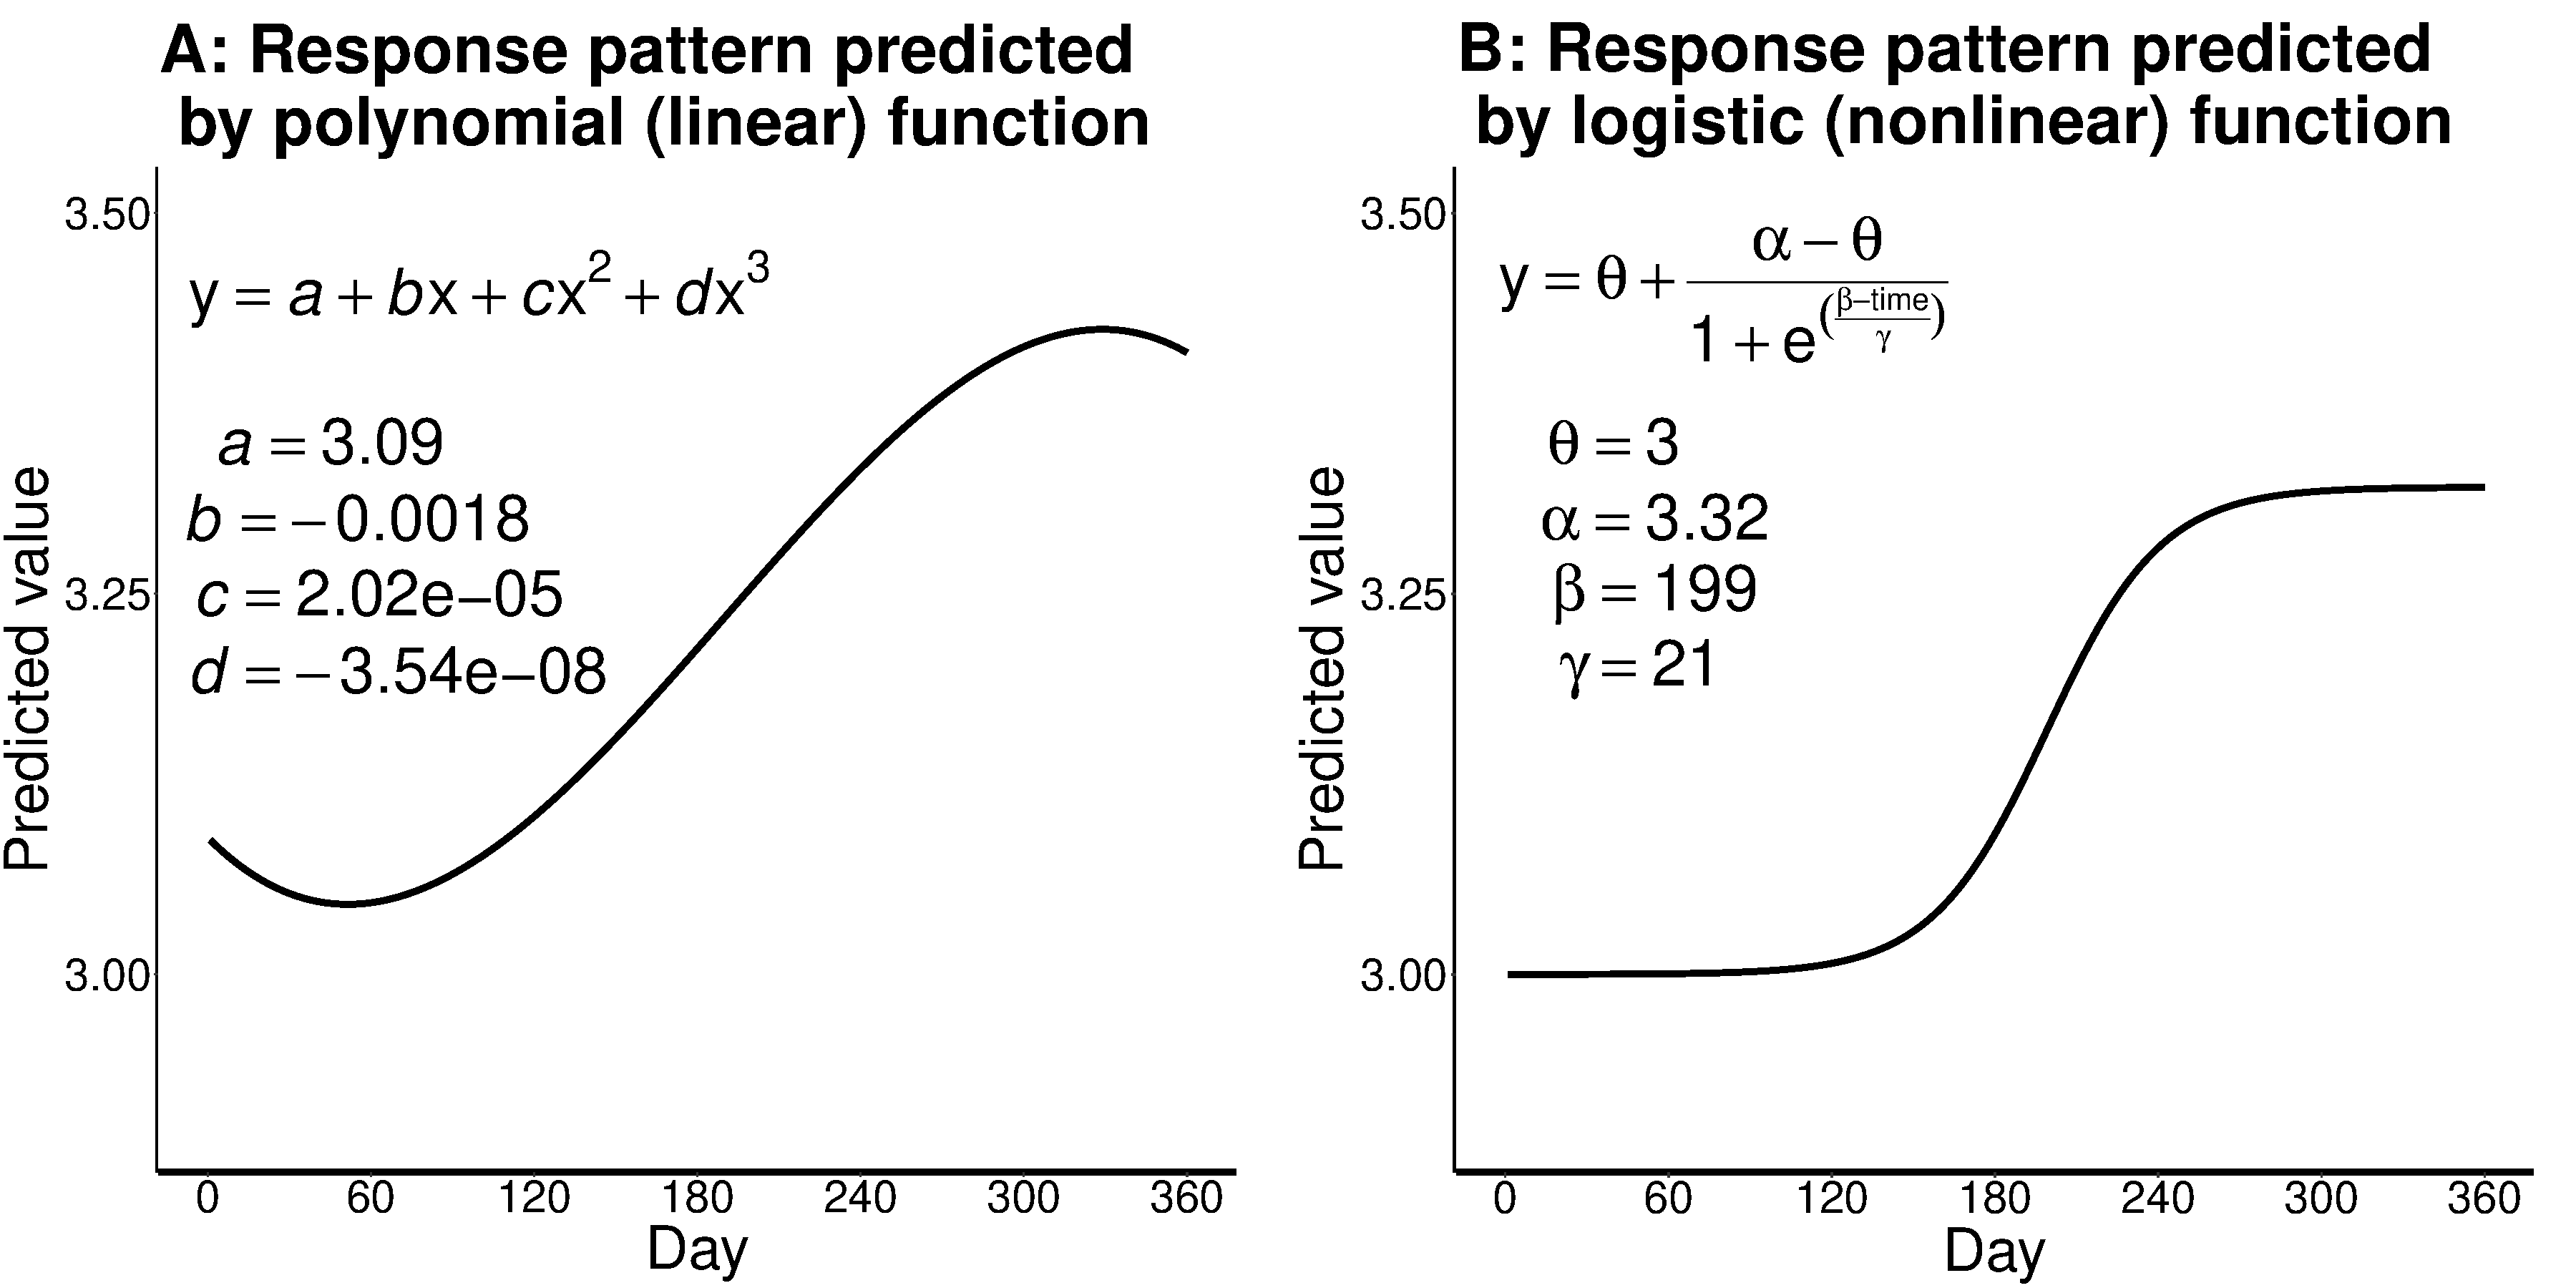
\includegraphics{Figures/polynomial_vs_nonlinear_plot} \hfill{}
  \figurefootnote{Panel A: Response pattern predicted by the polynomial function of Equation \eqref{eq:polynomial}. Panel B: Response pattern predicted by the logistic function of Equation \eqref{eq:logistic1}.}
\end{figure}

\hypertarget{overview-of-simulation-experiments}{%
\subsection{Overview of Simulation Experiments}\label{overview-of-simulation-experiments}}

To investigate the effects of longitudinal design and analysis factors on modelling accuracy, I conducted three Monte Carlo experiments. Before summarizing the simulation experiments, one point needs to be mentioned regarding the maximum number of independent variables used in each experiment. No simulation experiment manipulated more than three variables because of the difficulty associated with interpreting interactions between four or more variables. Even among academics, the ability to correctly interpret interactions sharply declines when the number of independent variables increases from three to four (Halford et al., 2005). Therefore, none of my simulation experiments manipulated more than three variables so that results could be readily interpreted.

To summarize the three simulation experiments, the independent variables of each simulation experiment are listed below:

\begin{itemize}
\tightlist
\item
  Experiment 1: number of measurements, spacing of measurements, and nature of change.
\item
  Experiment 2: number of measurements, spacing of measurements, and sample size.
\item
  Experiment 3: number of measurements, sample size, and time structuredness.
\end{itemize}

\noindent The sections that follow will present each of the simulation experiments and their corresponding results.

\begin{figure}[H]
  \caption{Description Each Parameters Logistic Function (Equation \ref{eq:logistic1})}
  \label{fig:combined_plot_1}
  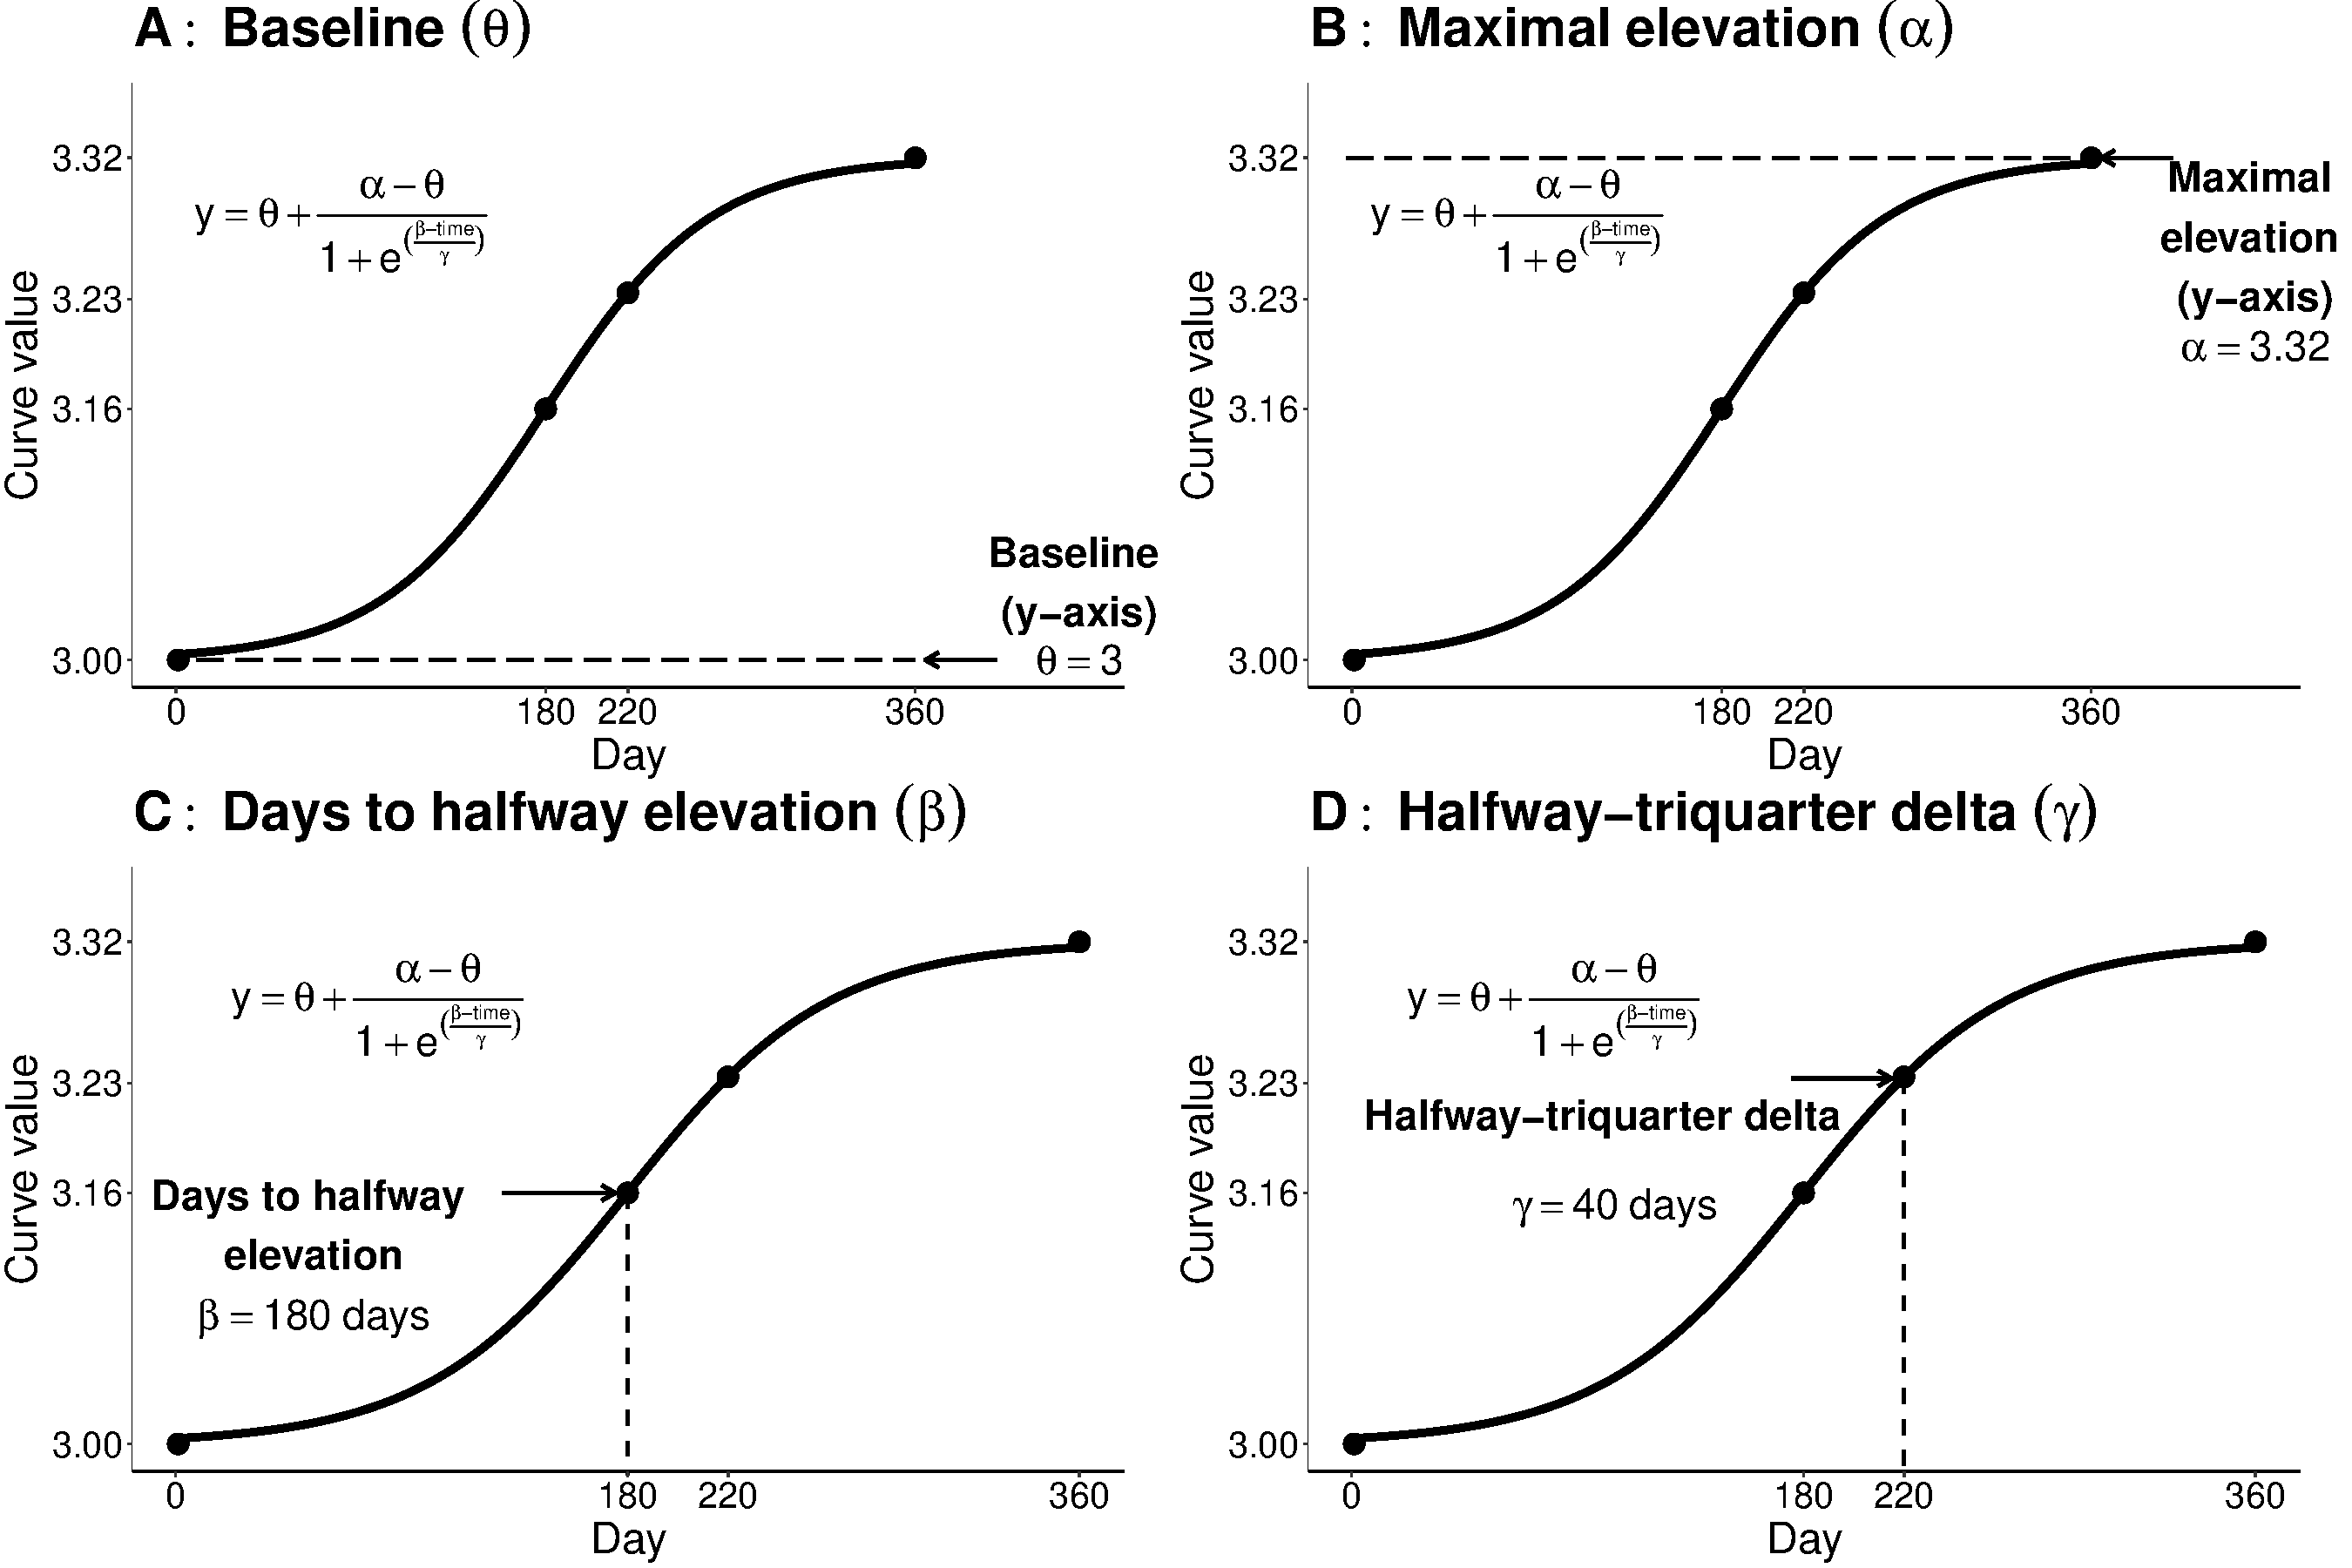
\includegraphics{Figures/combined_plot} \hfill{}
  \figurefootnote{Panel A: The baseline parameter ($\uptheta$) sets the starting value of the of curve, which in the current example has a value of 3.00 ($\uptheta$ = 3.00). Panel B: The maximal elevation parameter ($\upalpha$) sets the ending value of the curve, which in the current example has a value of 3.32 ($\upalpha$ = 3.32). Panel C: The days-to-halfway elevation parameter ($\upbeta$) sets the number of days needed to reach 50\% of the difference between the baseline and maximal elevation. In the current example, the baseline-maximal elevation difference is 0.32 ($\upalpha - \uptheta$ = 3.32 - 3.00 = 0.32), and so the days-to-halfway elevation parameter defines the number of days needed to reach a value of 3.16. Given that the days-to-halfway elevation parameter is set to 180 in the current example ($\upbeta = 180$), then 180 days are neededto go from a value of 3.00 to a value of 3.16. Panel D: The halfway-triquarter delta parameter ($\upgamma$) sets the number of days needed to go from halfway elevation to approximately 73\% of the baseline-maximal elevation difference of 0.32 ($\upalpha - \uptheta$ = 3.32 - 3.00 = 0.32). Given that 73\% of the baseline-maximal elevation difference is 0.23 and the halfway-triquarter delta is set to 40 days ($\upgamma = 40$), then 40 days are needed to go from the halfway point of 3.16 to the triquarter point of approximately 3.23).}
\end{figure}

\newpage
\vspace*{-\topskip}
\vspace*{\fill}
\nointerlineskip

\hypertarget{refs}{}
\begin{CSLReferences}{1}{0}
\leavevmode\vadjust pre{\hypertarget{ref-aguinis2021}{}}%
Aguinis, H., \& Bakker, R. M. (2021). Time is of the essence: Improving the conceptualization and measurement of time. \emph{Human Resource Management Review}, \emph{31}(2), 100763. \url{https://doi.org/10.1016/j.hrmr.2020.100763}

\leavevmode\vadjust pre{\hypertarget{ref-aydin2014}{}}%
Aydin, B., Leite, W. L., \& Algina, J. (2014). The Consequences of ignoring variability in measurement occasions within data collection waves in latent growth ,odels. \emph{Multivariate Behavioral Research}, \emph{49}(2), 149--160. \url{https://doi.org/10.1080/00273171.2014.887901}

\leavevmode\vadjust pre{\hypertarget{ref-baron1986}{}}%
Baron, R. M., \& Kenny, D. A. (1986). The moderator{\textendash}mediator variable distinction in social psychological research: Conceptual, strategic, and statistical considerations. \emph{Journal of Personality and Social Psychology}, \emph{51}(6), 1173--1182. \url{https://doi.org/10.1037/0022-3514.51.6.1173}

\leavevmode\vadjust pre{\hypertarget{ref-bauer2003}{}}%
Bauer, D. J. (2003). Estimating multilevel linear models as structural equation models. \emph{Journal of Educational and Behavioral Statistics}, \emph{28}(2), 135--167. \url{https://doi.org/10.3102/10769986028002135}

\leavevmode\vadjust pre{\hypertarget{ref-beal2015}{}}%
Beal, D. J. (2015). ESM 2.0: State of the art and future potential of experience sampling methods in organizational research. \emph{Annual Review of Organizational Psychology and Organizational Behavior}, \emph{2}(1), 383--407. \url{https://doi.org/10.1146/annurev-orgpsych-032414-111335}

\leavevmode\vadjust pre{\hypertarget{ref-bergman1993}{}}%
Bergman, L., \& Magnusson, D. (1990). \emph{General issues about data quality in longitudinal research} (L. Bergman \& D. Magnusson, Eds.; pp. 1--31). Cambridge University Press. \href{https://shorturl.at/enwxM}{shorturl.at/enwxM}

\leavevmode\vadjust pre{\hypertarget{ref-bodenmann2010}{}}%
Bodenmann, G., Atkins, D. C., Schär, M., \& Poffet, V. (2010). The association between daily stress and sexual activity. \emph{Journal of Family Psychology}, \emph{24}(3), 271--279. \url{https://doi.org/10.1037/a0019365}

\leavevmode\vadjust pre{\hypertarget{ref-burchinal1991}{}}%
Burchinal, M., \& Appelbaum, M. I. (1991). Estimating individual developmental functions: Methods and their assumptions. \emph{Child Development}, \emph{62}(1), 23. \url{https://doi.org/10.2307/1130702}

\leavevmode\vadjust pre{\hypertarget{ref-chen2014}{}}%
Chen, C. X., Martin, M., \& Merchant, K. A. (2014). The effect of measurement timing on the information content of customer satisfaction measures. \emph{Management Accounting Research}, \emph{25}(3), 187--205. \url{https://doi.org/10.1016/j.mar.2013.12.003}

\leavevmode\vadjust pre{\hypertarget{ref-cohen1993}{}}%
Cohen, A. (1993). Organizational commitment and turnover: A meta-analysis. \emph{Academy of Management Journal}, \emph{36}(5), 1140--1157. \url{https://doi.org/10.2307/256650}

\leavevmode\vadjust pre{\hypertarget{ref-cole2009}{}}%
Cole, D. A., \& Maxwell, S. E. (2009). Statistical methods for risk-outcome research: Being sensitive to longitudinal structure. \emph{Annual Review of Clinical Psychology}, \emph{5}(1), 71--96. \url{https://doi.org/10.1146/annurev-clinpsy-060508-130357}

\leavevmode\vadjust pre{\hypertarget{ref-cole2003}{}}%
Cole, D. A., \& Maxwell, S. E. (2003). Testing mediational models with longitudinal data: Questions and tips in the use of structural equation modeling. \emph{Journal of Abnormal Psychology}, \emph{112}(4), 558--577. \url{https://doi.org/10.1037/0021-843x.112.4.558}

\leavevmode\vadjust pre{\hypertarget{ref-collins2006}{}}%
Collins, L. M. (2006). Analysis of longitudinal data: The integration of theoretical model, temporal design, and statistical model. \emph{Annual Review of Psychology}, \emph{57}(1), 505--528. \url{https://doi.org/10.1146/annurev.psych.57.102904.190146}

\leavevmode\vadjust pre{\hypertarget{ref-coulombe2016b}{}}%
Coulombe, P. (2016). \emph{Partially and fully time-unstructured residual variance-covariance matrices in growth curve modeling: Consequences of ignoring variability in times of assessment} (Publication No. 10155460). {[}Doctoral dissertation, University of New Mexico{]}; {ProQuest Dissertations and Theses Global.}

\leavevmode\vadjust pre{\hypertarget{ref-coulombe2016}{}}%
Coulombe, P., Selig, J. P., \& Delaney, H. D. (2016). Ignoring individual differences in times of assessment in growth curve modeling. \emph{International Journal of Behavioral Development}, \emph{40}(1), 76--86. \url{https://doi.org/10.1177/0165025415577684}

\leavevmode\vadjust pre{\hypertarget{ref-cudeck2007}{}}%
Cudeck, R., \& Harring, J. R. (2007). Analysis of nonlinear patterns of change with random coefficient models. \emph{Annual Review of Psychology}, \emph{58}(1), 615--637. \url{https://doi.org/10.1146/annurev.psych.58.110405.085520}

\leavevmode\vadjust pre{\hypertarget{ref-curran2011}{}}%
Curran, P. J., \& Bauer, D. J. (2011). The disaggregation of within-person and between-person effects in longitudinal models of change. \emph{Annual Review of Psychology}, \emph{62}(1), 583--619. \url{https://doi.org/10.1146/annurev.psych.093008.100356}

\leavevmode\vadjust pre{\hypertarget{ref-dalal2014}{}}%
Dalal, R. S., Bhave, D. P., \& Fiset, J. (2014). Within-person variability in job performance. \emph{Journal of Management}, \emph{40}(5), 1396--1436. \url{https://doi.org/10.1177/0149206314532691}

\leavevmode\vadjust pre{\hypertarget{ref-day2011}{}}%
Day, D. V., \& Sin, H.-P. (2011). Longitudinal tests of an integrative model of leader development: Charting and understanding developmental trajectories. \emph{The Leadership Quarterly}, \emph{22}(3), 545--560. \url{https://doi.org/10.1016/j.leaqua.2011.04.011}

\leavevmode\vadjust pre{\hypertarget{ref-dillman2014}{}}%
Dillman, D. A., Smyth, J. D., \& Christian, L. M. (2014). \emph{Internet, phone, mail, and mixed-mode surveys: The tailored design method}. John Wiley \& Sons.

\leavevmode\vadjust pre{\hypertarget{ref-dormann2015}{}}%
Dormann, C., \& Griffin, M. A. (2015). Optimal time lags in panel studies. \emph{Psychological Methods}, \emph{20}(4), 489--505. \url{https://doi.org/10.1037/met0000041}

\leavevmode\vadjust pre{\hypertarget{ref-dormann2014}{}}%
Dormann, C., \& Ven, B. van de. (2014). Timing in methods for studying psychosocial factors at work. In \emph{Psychosocial factors at work in the asia pacific} (1st ed., pp. 89--116). Springer Dordrecht. \url{https://doi.org/10.1007/978-94-017-8975-2_4}

\leavevmode\vadjust pre{\hypertarget{ref-enders2007}{}}%
Enders, C. K., \& Tofighi, D. (2007). Centering predictor variables in cross-sectional multilevel models: A new look at an old issue. \emph{Psychological Methods}, \emph{12}(2), 121--138. \url{https://doi.org/10.1037/1082-989x.12.2.121}

\leavevmode\vadjust pre{\hypertarget{ref-finch2017}{}}%
Finch, W. H. (2017). Investigation of parameter estimation accuracy for growth curve modeling with categorical indicators. \emph{Methodology}, \emph{13}(3), 98--112. \url{https://doi.org/10.1027/1614-2241/a000134}

\leavevmode\vadjust pre{\hypertarget{ref-fine2020}{}}%
Fine, K. L., \& Grimm, K. J. (2020). Examination of nonlinear and functional mixed-effects models with nonparametrically generated data. \emph{Multivariate Behavioral Research}, 1--18. \url{https://doi.org/10.1080/00273171.2020.1754746}

\leavevmode\vadjust pre{\hypertarget{ref-fine2019}{}}%
Fine, K. L., Suk, H. W., \& Grimm, K. J. (2019). An examination of a functional mixed-effects modeling approach to the analysis of longitudinal data. \emph{Multivariate Behavioral Research}, \emph{54}(4), 475--491. \url{https://doi.org/10.1080/00273171.2018.1520626}

\leavevmode\vadjust pre{\hypertarget{ref-fisher2008}{}}%
Fisher, C. D. (2008). What if we took within-person variability seriously? \emph{Industrial and Organizational Psychology}, \emph{1}(2), 185--189. \url{https://doi.org/10.1111/j.1754-9434.2008.00036.x}

\leavevmode\vadjust pre{\hypertarget{ref-fisher2018}{}}%
Fisher, J., Medaglia, J. D., \& Jeronimus, B. F. (2018). Lack of group-to-individual generalizability is a threat to human subjects research. \emph{Proceedings of the National Academy of Sciences}, \emph{115}(27). \url{https://doi.org/10.1073/pnas.1711978115}

\leavevmode\vadjust pre{\hypertarget{ref-fournier2017}{}}%
Fournier, M., d'Arripe-Longueville, F., Rovere, C., Easthope, C. S., Schwabe, L., El Methni, J., \& Radel, R. (2017). Effects of circadian cortisol on the development of a health habit. \emph{Health Psychology}, \emph{36}(11), 1059--1064. \url{https://doi.org/10.1037/hea0000510}

\leavevmode\vadjust pre{\hypertarget{ref-fried2004}{}}%
Fried, Y., \& Slowik, L. H. (2004). Enriching goal-setting theory with time: An integrated approach. \emph{Academy of Management Review}, \emph{29}(3), 404--422. \url{https://doi.org/10.5465/amr.2004.13670973}

\leavevmode\vadjust pre{\hypertarget{ref-gasimova2014}{}}%
Gasimova, F., Robitzsch, A., Wilhelm, O., \& Hülür, G. (2014). A Hierarchical bayesian model with correlated residuals for investigating stability and change in intensive longitudinal data settings. \emph{Methodology}, \emph{10}(4), 126--137. \url{https://doi.org/10.1027/1614-2241/a000083}

\leavevmode\vadjust pre{\hypertarget{ref-george2000}{}}%
George, J. M., \& Jones, G. R. (2000). The role of time in theory and theory building. \emph{Journal of Management}, \emph{26}(4), 657--684. \url{https://doi.org/10.1177/014920630002600404}

\leavevmode\vadjust pre{\hypertarget{ref-griffeth2000}{}}%
Griffeth, R. W., Hom, P. W., \& Gaertner, S. (2000). A meta-analysis of antecedents and correlates of employee turnover: Update, moderator tests, and research implications for the next millennium. \emph{Journal of Management}, \emph{26}(3), 463--488. \url{https://doi.org/10.1177/014920630002600305}

\leavevmode\vadjust pre{\hypertarget{ref-grimm2010a}{}}%
Grimm, K., \& Widaman, K. (2010). Residual structures in latent growth curve modeling. \emph{Structural Equation Modeling: A Multidisciplinary Journal}, \emph{17}(3), 424--442. \url{https://doi.org/10.1080/10705511.2010.489006}

\leavevmode\vadjust pre{\hypertarget{ref-halford2005}{}}%
Halford, G. S., Baker, R., McCredden, J. E., \& Bain, J. D. (2005). How many variables can humans process? \emph{Psychological Science}, \emph{16}(1), 70--76. \url{https://doi.org/10.1111/j.0956-7976.2005.00782.x}

\leavevmode\vadjust pre{\hypertarget{ref-hamaker2005}{}}%
Hamaker, E. L., Dolan, C. V., \& Molenaar, P. C. M. (2005). Statistical modeling of the individual: Rationale and application of multivariate stationary time series analysis. \emph{Multivariate Behavioral Research}, \emph{40}(2), 207--233. \url{https://doi.org/10.1207/s15327906mbr4002_3}

\leavevmode\vadjust pre{\hypertarget{ref-hom1992}{}}%
Hom, P. W., Caranikas-Walker, F., Prussia, G. E., \& Griffeth, R. W. (1992). A meta-analytical structural equations analysis of a model of employee turnover. \emph{Journal of Applied Psychology}, \emph{77}(6), 890--909. \url{https://doi.org/10.1037/0021-9010.77.6.890}

\leavevmode\vadjust pre{\hypertarget{ref-huh2015}{}}%
Huh, D., Kaysen, D. L., \& Atkins, D. C. (2015). Modeling cyclical patterns in daily college drinking data with many zeroes. \emph{Multivariate Behavioral Research}, \emph{50}(2), 184--196. \url{https://doi.org/10.1080/00273171.2014.977433}

\leavevmode\vadjust pre{\hypertarget{ref-kenny2014}{}}%
Kenny, D. A., \& Judd, C. M. (2014). Power anomalies in testing mediation. \emph{Psychological Science}, \emph{25}(2), 334--339. \url{https://doi.org/10.1177/0956797613502676}

\leavevmode\vadjust pre{\hypertarget{ref-kunisch2017}{}}%
Kunisch, S., Bartunek, J. M., Mueller, J., \& Huy, Q. N. (2017). Time in strategic change research. \emph{Academy of Management Annals}, \emph{11}(2), 1005--1064. \url{https://doi.org/10.5465/annals.2015.0133}

\leavevmode\vadjust pre{\hypertarget{ref-larsen1990}{}}%
Larsen, R. J., \& Kasimatis, M. (1990). Individual differences in entrainment of mood to the weekly calendar. \emph{Journal of Personality and Social Psychology}, \emph{58}(1), 164--171. \url{https://doi.org/10.1037/0022-3514.58.1.164}

\leavevmode\vadjust pre{\hypertarget{ref-lawrence2001}{}}%
Lawrence, T. B., Winn, M. I., \& Jennings, P. D. (2001). The temporal dynamics of institutionalization. \emph{Academy of Management Review}, \emph{26}(4), 624--644. \url{https://doi.org/10.5465/amr.2001.5393901}

\leavevmode\vadjust pre{\hypertarget{ref-liu2021}{}}%
Liu, J., \& Perera, R. A. (2021). Estimating knots and their association in parallel bilinear spline growth curve models in the framework of individual measurement occasions. \emph{Psychological Methods}. \url{https://doi.org/10.1037/met0000309}

\leavevmode\vadjust pre{\hypertarget{ref-liu2019}{}}%
Liu, J., Perera, R. A., Kang, L., Kirkpatrick, R. M., \& Sabo, R. T. (2019). Obtaining interpretable parameters from reparameterizing longitudinal models: Transformation matrices between growth factors in two parameter-spaces. \emph{arXiv Preprint arXiv:1911.09939}.

\leavevmode\vadjust pre{\hypertarget{ref-liu2015}{}}%
Liu, Y., Liu, H., Li, H., \& Zhao, Q. (2015). The effects of individually varying times of observations on growth parameter estimations in piecewise growth model. \emph{Journal of Applied Statistics}, \emph{42}(9), 1843--1860. \url{https://doi.org/10.1080/02664763.2015.1014884}

\leavevmode\vadjust pre{\hypertarget{ref-maxwell2007}{}}%
Maxwell, S. E., \& Cole, D. A. (2007). Bias in cross-sectional analyses of longitudinal mediation. \emph{Psychological Methods}, \emph{12}(1), 23--44. \url{https://doi.org/10.1037/1082-989x.12.1.23}

\leavevmode\vadjust pre{\hypertarget{ref-maxwell2011}{}}%
Maxwell, S. E., Cole, D. A., \& Mitchell, M. A. (2011). Bias in cross-sectional analyses of longitudinal mediation: Partial and complete mediation under an autoregressive model. \emph{Multivariate Behavioral Research}, \emph{46}(5), 816--841. \url{https://doi.org/10.1080/00273171.2011.606716}

\leavevmode\vadjust pre{\hypertarget{ref-mehta2005}{}}%
Mehta, P. D., \& Neale, M. C. (2005). People are variables too: Multilevel structural equations modeling. \emph{Psychological Methods}, \emph{10}(3), 259--284. \url{https://doi.org/10.1037/1082-989x.10.3.259}

\leavevmode\vadjust pre{\hypertarget{ref-mehta2000}{}}%
Mehta, P. D., \& West, S. G. (2000). Putting the individual back into individual growth curves. \emph{Psychological Methods}, \emph{5}(1), 23--43. \url{https://doi.org/10.1037/1082-989x.5.1.23}

\leavevmode\vadjust pre{\hypertarget{ref-mill2011}{}}%
Mill, J. S. (2011). Of the law of universal causation. In \emph{A system of logic, tatiocinative and inductive: Being a connected view of the principles of evidence, and the methods of scientific investigation} (Vol. 1, pp. 392--424). Cambridge University Press. (Original work published in 1843). \url{https://doi.org/10.1017/cbo9781139149839.021}

\leavevmode\vadjust pre{\hypertarget{ref-miller2017}{}}%
Miller, M. L., \& Ferrer, E. (2017). The effect of sampling-time variation on latent growth curve models. \emph{Structural Equation Modeling: A Multidisciplinary Journal}, \emph{24}(6), 831--854. \url{https://doi.org/10.1080/10705511.2017.1346476}

\leavevmode\vadjust pre{\hypertarget{ref-mitchell2013}{}}%
Mitchell, M. A., \& Maxwell, S. E. (2013). A comparison of the cross-sectional and sequential designs when assessing longitudinal mediation. \emph{Multivariate Behavioral Research}, \emph{48}(3), 301--339. \url{https://doi.org/10.1080/00273171.2013.784696}

\leavevmode\vadjust pre{\hypertarget{ref-mitchell2001}{}}%
Mitchell, T. R., \& James, L. R. (2001). Building better theory: Time and the specification of when things happen. \emph{Academy of Management Review}, \emph{26}(4), 530--547. \url{https://doi.org/10.5465/amr.2001.5393889}

\leavevmode\vadjust pre{\hypertarget{ref-wang2007}{}}%
Mo Wang, \& Bodner, T. E. (2007). Growth mixture modeling. \emph{Organizational Research Methods}, \emph{10}(4), 635--656. \url{https://doi.org/10.1177/1094428106289397}

\leavevmode\vadjust pre{\hypertarget{ref-molenaar2004}{}}%
Molenaar, P. C. M. (2004). A manifesto on psychology as idiographic science: Bringing the person back into scientific psychology, this time forever. \emph{Measurement: Interdisciplinary Research \& Perspective}, \emph{2}(4), 201--218. \url{https://doi.org/10.1207/s15366359mea0204_1}

\leavevmode\vadjust pre{\hypertarget{ref-molenaar2009}{}}%
Molenaar, P. C. M., \& Campbell, C. G. (2009). The new person-specific paradigm in psychology. \emph{Current Directions in Psychological Science}, \emph{18}(2), 112--117. \url{https://doi.org/10.1111/j.1467-8721.2009.01619.x}

\leavevmode\vadjust pre{\hypertarget{ref-murphy2011}{}}%
Murphy, D. L., Beretvas, S. N., \& Pituch, K. A. (2011). The effects of autocorrelation on the curve-of-factors growth model. \emph{Structural Equation Modeling: A Multidisciplinary Journal}, \emph{18}(3), 430--448. \url{https://doi.org/10.1080/10705511.2011.582399}

\leavevmode\vadjust pre{\hypertarget{ref-murre2015}{}}%
Murre, J. M. J., \& Dros, J. (2015). Replication and analysis of Ebbinghaus{'} forgetting curve. \emph{PLOS ONE}, \emph{10}(7), e0120644. \url{https://doi.org/10.1371/journal.pone.0120644}

\leavevmode\vadjust pre{\hypertarget{ref-navarro2015}{}}%
Navarro, J., Roe, R. A., \& Artiles, M. I. (2015). Taking time seriously: Changing practices and perspectives in work/organizational psychology. \emph{Journal of Work and Organizational Psychology}, \emph{31}(3), 135--145. \url{https://doi.org/10.1016/j.rpto.2015.07.002}

\leavevmode\vadjust pre{\hypertarget{ref-nederhof1985}{}}%
Nederhof, A. J. (1985). Methods of coping with social desirability bias: A review. \emph{European Journal of Social Psychology}, \emph{15}(3), 263--280. \url{https://doi.org/10.1002/ejsp.2420150303}

\leavevmode\vadjust pre{\hypertarget{ref-newman2008}{}}%
Newman, D. A. (2008). \emph{Missing data techniques and low response rates: The role of systematic nonresponse parameters} (C. E. Lance \& R. J. Vandenberg, Eds.; pp. 7--36). Routledge. \url{https://doi.org/10.4324/9780203867266}

\leavevmode\vadjust pre{\hypertarget{ref-newsom2020}{}}%
Newsom, J. T., \& Smith, N. A. (2020). Performance of latent growth curve models with binary variables. \emph{Structural Equation Modeling: A Multidisciplinary Journal}, \emph{27}(6), 888--907. \url{https://doi.org/10.1080/10705511.2019.1705825}

\leavevmode\vadjust pre{\hypertarget{ref-nixon2011}{}}%
Nixon, A. E., Mazzola, J. J., Bauer, J., Krueger, J. R., \& Spector, P. E. (2011). Can work make you sick? A meta-analysis of the relationships between job stressors and physical symptoms. \emph{Work \& Stress}, \emph{25}(1), 1--22. \url{https://doi.org/10.1080/02678373.2011.569175}

\leavevmode\vadjust pre{\hypertarget{ref-olaughlin2018}{}}%
O'Laughlin, K. D., Martin, M. J., \& Ferrer, E. (2018). Cross-sectional analysis of longitudinal mediation processes. \emph{Multivariate Behavioral Research}, \emph{53}(3), 375--402. \url{https://doi.org/10.1080/00273171.2018.1454822}

\leavevmode\vadjust pre{\hypertarget{ref-orourke2021}{}}%
O'Rourke, H. P., Fine, K. L., Grimm, K. J., \& MacKinnon, D. P. (2021). The Importance of time metric precision when implementing bivariate latent change score ,odels. \emph{Multivariate Behavioral Research}, 1--19. \url{https://doi.org/10.1080/00273171.2021.1874261}

\leavevmode\vadjust pre{\hypertarget{ref-orne1962}{}}%
Orne, M. T. (1962). On the social psychology of the psychological experiment: With particular reference to demand characteristics and their implications. \emph{American Psychologist}, \emph{17}(11), 776--783. \url{https://doi.org/10.1037/h0043424}

\leavevmode\vadjust pre{\hypertarget{ref-ostroff2002}{}}%
Ostroff, C., Kinicki, A. J., \& Clark, M. A. (2002). Substantive and operational issues of response bias across levels of analysis: An example of climate-satisfaction relationships. \emph{Journal of Applied Psychology}, \emph{87}(2), 355--368. \url{https://doi.org/10.1037/0021-9010.87.2.355}

\leavevmode\vadjust pre{\hypertarget{ref-ployhart2010}{}}%
Ployhart, R. E., \& Vandenberg, R. J. (2010). Longitudinal research: The theory, design, and analysis of change. \emph{Journal of Management}, \emph{36}(1), 94--120. \url{https://doi.org/10.1177/0149206309352110}

\leavevmode\vadjust pre{\hypertarget{ref-podsakoff2003}{}}%
Podsakoff, P. M., MacKenzie, S. B., Lee, J.-Y., \& Podsakoff, N. P. (2003). Common method biases in behavioral research: A critical review of the literature and recommended remedies. \emph{Journal of Applied Psychology}, \emph{88}(5), 879--903. \url{https://doi.org/10.1037/0021-9010.88.5.879}

\leavevmode\vadjust pre{\hypertarget{ref-ram2013}{}}%
Ram, N., Brose, A., \& Molenaar, P. C. M. (2013). \emph{Dynamic factor analysis: Modeling person-specific process} (T. D. Little, Ed.; Vol. 2, pp. 441--457). Oxford University Press. \url{https://doi.org/10.1093/oxfordhb/9780199934898.013.0021}

\leavevmode\vadjust pre{\hypertarget{ref-raudenbush2002}{}}%
Raudenbush, S. W., \& Bryk, A. S. (2002). \emph{Hierarchical linear models: Applications and data analysis methods} (2nd ed., Vol. 1). SAGE Publications. \href{https://shorturl.at/imFN7}{shorturl.at/imFN7}

\leavevmode\vadjust pre{\hypertarget{ref-riketta2008}{}}%
Riketta, M. (2008). The causal relation between job attitudes and performance: A meta-analysis of panel studies. \emph{Journal of Applied Psychology}, \emph{93}(2), 472--481. \url{https://doi.org/10.1037/0021-9010.93.2.472}

\leavevmode\vadjust pre{\hypertarget{ref-robert2010}{}}%
Robert, C., \& Casella, G. (2010). \emph{Introducing monte carlo methods with r} (1st ed.). Springer New York. \url{https://doi.org/10.1007/978-1-4419-1576-4}

\leavevmode\vadjust pre{\hypertarget{ref-roe2008}{}}%
Roe, R. A. (2008). Time in applied psychology. \emph{European Psychologist}, \emph{13}(1), 37--52. \url{https://doi.org/10.1027/1016-9040.13.1.37}

\leavevmode\vadjust pre{\hypertarget{ref-roe2014}{}}%
Roe, R. A. (2014). Test validity from a temporal perspective: Incorporating time in validation research. \emph{European Journal of Work and Organizational Psychology}, \emph{23}(5), 754--768. \url{https://doi.org/10.1080/1359432x.2013.804177}

\leavevmode\vadjust pre{\hypertarget{ref-roe2012}{}}%
Roe, R. A., Gockel, C., \& Meyer, B. (2012). Time and change in teams: Where we are and where we are moving. \emph{European Journal of Work and Organizational Psychology}, \emph{21}(5), 629--656. \url{https://doi.org/10.1080/1359432x.2012.729821}

\leavevmode\vadjust pre{\hypertarget{ref-vandeschoot2012}{}}%
Schoot, R. van de, Lugtig, P., \& Hox, J. (2012). A checklist for testing measurement invariance. \emph{European Journal of Developmental Psychology}, \emph{9}(4), 486--492. \url{https://doi.org/10.1080/17405629.2012.686740}

\leavevmode\vadjust pre{\hypertarget{ref-shipp2015}{}}%
Shipp, A. J., \& Cole, M. S. (2015). Time in individual-level organizational studies: What is it, how is it used, and why isn{'}t it exploited more often? \emph{Annual Review of Organizational Psychology and Organizational Behavior}, \emph{2}(1), 237--260. \url{https://doi.org/10.1146/annurev-orgpsych-032414-111245}

\leavevmode\vadjust pre{\hypertarget{ref-sonnentag2012}{}}%
Sonnentag, S. (2012). Time in organizational research: Catching up on a long neglected topic in order to improve theory. \emph{Organizational Psychology Review}, \emph{2}(4), 361--368. \url{https://doi.org/10.1177/2041386612442079}

\leavevmode\vadjust pre{\hypertarget{ref-stanley2014}{}}%
Stanley, D. J., \& Spence, J. R. (2014). Expectations for eeplications. \emph{Perspectives on Psychological Science}, \emph{9}(3), 305--318. \url{https://doi.org/10.1177/1745691614528518}

\leavevmode\vadjust pre{\hypertarget{ref-steel1990}{}}%
Steel, R. P., Hendrix, W. H., \& Balogh, S. P. (1990). Confounding effects of the turnover base rate on relations between time lag and turnover study outcomes: An extension of meta-analysis findings and conclusions. \emph{Journal of Organizational Behavior}, \emph{11}(3), 237--242. \url{https://doi.org/10.1002/job.4030110306}

\leavevmode\vadjust pre{\hypertarget{ref-steel1984}{}}%
Steel, R. P., \& Ovalle, N. K. (1984). A review and meta-analysis of research on the relationship between behavioral intentions and employee turnover. \emph{Journal of Applied Psychology}, \emph{69}(4), 673--686. \url{https://doi.org/10.1037/0021-9010.69.4.673}

\leavevmode\vadjust pre{\hypertarget{ref-stockdale2007}{}}%
Stockdale, G. D. (2007). \emph{Factors affecting goodness of fit of the quasi-simplex, linear growth curve, and latent difference score models to oppositive data structures: A simulation study} (Publication No. 3303209). {[}Doctoral dissertation, University of California{]}; {ProQuest Dissertations and Theses Global.}

\leavevmode\vadjust pre{\hypertarget{ref-tiberio2008}{}}%
Tiberio, S. S. (2008). \emph{The effects of misspecified measurement intervals in multivariate latent differential equation models} (Publication No. 3441759). {[}Doctoral dissertation, University of Notre Dame{]}; {ProQuest Dissertations and Theses Global.}

\leavevmode\vadjust pre{\hypertarget{ref-timmons2015}{}}%
Timmons, A. C., \& Preacher, K. J. (2015). The importance of temporal design: How do measurement intervals affect the accuracy and efficiency of parameter estimates in longitudinal research? \emph{Multivariate Behavioral Research}, \emph{50}(1), 41--55. \url{https://doi.org/10.1080/00273171.2014.961056}

\leavevmode\vadjust pre{\hypertarget{ref-vantilborgh2018}{}}%
Vantilborgh, T., Hofmans, J., \& Judge, T. A. (2018). The time has come to study dynamics at work. In \emph{Journal of Organizational Behavior} (No. 9; Vol. 39, pp. 1045--1049). Wiley Online Library. \url{https://doi.org/10.1002/job.2327}

\leavevmode\vadjust pre{\hypertarget{ref-wang2015}{}}%
Wang, L. (Peggy)., \& Maxwell, S. E. (2015). On disaggregating between-person and within-person effects with longitudinal data using multilevel models. \emph{Psychological Methods}, \emph{20}(1), 63--83. \url{https://doi.org/10.1037/met0000030}

\leavevmode\vadjust pre{\hypertarget{ref-whetten1989}{}}%
Whetten, D. A. (1989). What constitutes a theoretical contribution? \emph{Academy of Management Review}, \emph{14}(4), 490--495. \url{https://doi.org/10.5465/amr.1989.4308371}

\leavevmode\vadjust pre{\hypertarget{ref-wu2014}{}}%
Wu, J.-Y., Kwok, O.-M., \& Willson, V. (2014). Using design-based latent growth curve modeling with cluster-level predictor to address dependency. \emph{The Journal of Experimental Education}, \emph{82}(4), 431--454. \url{https://doi.org/10.1080/00220973.2013.876226}

\leavevmode\vadjust pre{\hypertarget{ref-wu2017}{}}%
Wu, W., Jia, F., Kinai, R., \& Little, T. D. (2016). Optimal number and allocation of data collection points for linear spline growth curve modeling. \emph{International Journal of Behavioral Development}, \emph{41}(4), 550--558. \url{https://doi.org/10.1177/0165025416644076}

\leavevmode\vadjust pre{\hypertarget{ref-xia2020}{}}%
Xia, W., Ye, M., Liu, J., Cao, M., \& Sun, X.-M. (2020). Analysis of a nonlinear opinion dynamics model with biased assimilation. \emph{Automatica}, \emph{120}, 109113. \url{https://doi.org/10.1016/j.automatica.2020.109113}

\leavevmode\vadjust pre{\hypertarget{ref-ye2016}{}}%
Ye, F. (2016). Latent growth curve analysis with dichotomous items: Comparing four approaches. \emph{British Journal of Mathematical and Statistical Psychology}, \emph{69}(1), 43--61. \url{https://doi.org/10.1111/bmsp.12058}

\leavevmode\vadjust pre{\hypertarget{ref-zaheer1999}{}}%
Zaheer, S., Albert, S., \& Zaheer, A. (1999). Time scales and organizational theory. \emph{Academy of Management Review}, \emph{24}(4), 725--741. \url{https://doi.org/10.5465/amr.1999.2553250}

\end{CSLReferences}


\end{document}
